% Generated by Sphinx.
\def\sphinxdocclass{report}
\documentclass[letterpaper,10pt,english]{sphinxmanual}
\usepackage[utf8]{inputenc}
\DeclareUnicodeCharacter{00A0}{\nobreakspace}
\usepackage[T1]{fontenc}
\usepackage{babel}
\usepackage{times}
\usepackage[Bjarne]{fncychap}
\usepackage{longtable}
\usepackage{sphinx}
\usepackage{multirow}


\title{bioplot Documentation}
\date{January 12, 2015}
\release{1}
\author{drs. ing. J.S. Bouten}
\newcommand{\sphinxlogo}{}
\renewcommand{\releasename}{Release}
\makeindex

\makeatletter
\def\PYG@reset{\let\PYG@it=\relax \let\PYG@bf=\relax%
    \let\PYG@ul=\relax \let\PYG@tc=\relax%
    \let\PYG@bc=\relax \let\PYG@ff=\relax}
\def\PYG@tok#1{\csname PYG@tok@#1\endcsname}
\def\PYG@toks#1+{\ifx\relax#1\empty\else%
    \PYG@tok{#1}\expandafter\PYG@toks\fi}
\def\PYG@do#1{\PYG@bc{\PYG@tc{\PYG@ul{%
    \PYG@it{\PYG@bf{\PYG@ff{#1}}}}}}}
\def\PYG#1#2{\PYG@reset\PYG@toks#1+\relax+\PYG@do{#2}}

\def\PYG@tok@gd{\def\PYG@tc##1{\textcolor[rgb]{0.63,0.00,0.00}{##1}}}
\def\PYG@tok@gu{\let\PYG@bf=\textbf\def\PYG@tc##1{\textcolor[rgb]{0.50,0.00,0.50}{##1}}}
\def\PYG@tok@gt{\def\PYG@tc##1{\textcolor[rgb]{0.00,0.25,0.82}{##1}}}
\def\PYG@tok@gs{\let\PYG@bf=\textbf}
\def\PYG@tok@gr{\def\PYG@tc##1{\textcolor[rgb]{1.00,0.00,0.00}{##1}}}
\def\PYG@tok@cm{\let\PYG@it=\textit\def\PYG@tc##1{\textcolor[rgb]{0.25,0.50,0.56}{##1}}}
\def\PYG@tok@vg{\def\PYG@tc##1{\textcolor[rgb]{0.73,0.38,0.84}{##1}}}
\def\PYG@tok@m{\def\PYG@tc##1{\textcolor[rgb]{0.13,0.50,0.31}{##1}}}
\def\PYG@tok@mh{\def\PYG@tc##1{\textcolor[rgb]{0.13,0.50,0.31}{##1}}}
\def\PYG@tok@cs{\def\PYG@tc##1{\textcolor[rgb]{0.25,0.50,0.56}{##1}}\def\PYG@bc##1{\colorbox[rgb]{1.00,0.94,0.94}{##1}}}
\def\PYG@tok@ge{\let\PYG@it=\textit}
\def\PYG@tok@vc{\def\PYG@tc##1{\textcolor[rgb]{0.73,0.38,0.84}{##1}}}
\def\PYG@tok@il{\def\PYG@tc##1{\textcolor[rgb]{0.13,0.50,0.31}{##1}}}
\def\PYG@tok@go{\def\PYG@tc##1{\textcolor[rgb]{0.19,0.19,0.19}{##1}}}
\def\PYG@tok@cp{\def\PYG@tc##1{\textcolor[rgb]{0.00,0.44,0.13}{##1}}}
\def\PYG@tok@gi{\def\PYG@tc##1{\textcolor[rgb]{0.00,0.63,0.00}{##1}}}
\def\PYG@tok@gh{\let\PYG@bf=\textbf\def\PYG@tc##1{\textcolor[rgb]{0.00,0.00,0.50}{##1}}}
\def\PYG@tok@ni{\let\PYG@bf=\textbf\def\PYG@tc##1{\textcolor[rgb]{0.84,0.33,0.22}{##1}}}
\def\PYG@tok@nl{\let\PYG@bf=\textbf\def\PYG@tc##1{\textcolor[rgb]{0.00,0.13,0.44}{##1}}}
\def\PYG@tok@nn{\let\PYG@bf=\textbf\def\PYG@tc##1{\textcolor[rgb]{0.05,0.52,0.71}{##1}}}
\def\PYG@tok@no{\def\PYG@tc##1{\textcolor[rgb]{0.38,0.68,0.84}{##1}}}
\def\PYG@tok@na{\def\PYG@tc##1{\textcolor[rgb]{0.25,0.44,0.63}{##1}}}
\def\PYG@tok@nb{\def\PYG@tc##1{\textcolor[rgb]{0.00,0.44,0.13}{##1}}}
\def\PYG@tok@nc{\let\PYG@bf=\textbf\def\PYG@tc##1{\textcolor[rgb]{0.05,0.52,0.71}{##1}}}
\def\PYG@tok@nd{\let\PYG@bf=\textbf\def\PYG@tc##1{\textcolor[rgb]{0.33,0.33,0.33}{##1}}}
\def\PYG@tok@ne{\def\PYG@tc##1{\textcolor[rgb]{0.00,0.44,0.13}{##1}}}
\def\PYG@tok@nf{\def\PYG@tc##1{\textcolor[rgb]{0.02,0.16,0.49}{##1}}}
\def\PYG@tok@si{\let\PYG@it=\textit\def\PYG@tc##1{\textcolor[rgb]{0.44,0.63,0.82}{##1}}}
\def\PYG@tok@s2{\def\PYG@tc##1{\textcolor[rgb]{0.25,0.44,0.63}{##1}}}
\def\PYG@tok@vi{\def\PYG@tc##1{\textcolor[rgb]{0.73,0.38,0.84}{##1}}}
\def\PYG@tok@nt{\let\PYG@bf=\textbf\def\PYG@tc##1{\textcolor[rgb]{0.02,0.16,0.45}{##1}}}
\def\PYG@tok@nv{\def\PYG@tc##1{\textcolor[rgb]{0.73,0.38,0.84}{##1}}}
\def\PYG@tok@s1{\def\PYG@tc##1{\textcolor[rgb]{0.25,0.44,0.63}{##1}}}
\def\PYG@tok@gp{\let\PYG@bf=\textbf\def\PYG@tc##1{\textcolor[rgb]{0.78,0.36,0.04}{##1}}}
\def\PYG@tok@sh{\def\PYG@tc##1{\textcolor[rgb]{0.25,0.44,0.63}{##1}}}
\def\PYG@tok@ow{\let\PYG@bf=\textbf\def\PYG@tc##1{\textcolor[rgb]{0.00,0.44,0.13}{##1}}}
\def\PYG@tok@sx{\def\PYG@tc##1{\textcolor[rgb]{0.78,0.36,0.04}{##1}}}
\def\PYG@tok@bp{\def\PYG@tc##1{\textcolor[rgb]{0.00,0.44,0.13}{##1}}}
\def\PYG@tok@c1{\let\PYG@it=\textit\def\PYG@tc##1{\textcolor[rgb]{0.25,0.50,0.56}{##1}}}
\def\PYG@tok@kc{\let\PYG@bf=\textbf\def\PYG@tc##1{\textcolor[rgb]{0.00,0.44,0.13}{##1}}}
\def\PYG@tok@c{\let\PYG@it=\textit\def\PYG@tc##1{\textcolor[rgb]{0.25,0.50,0.56}{##1}}}
\def\PYG@tok@mf{\def\PYG@tc##1{\textcolor[rgb]{0.13,0.50,0.31}{##1}}}
\def\PYG@tok@err{\def\PYG@bc##1{\fcolorbox[rgb]{1.00,0.00,0.00}{1,1,1}{##1}}}
\def\PYG@tok@kd{\let\PYG@bf=\textbf\def\PYG@tc##1{\textcolor[rgb]{0.00,0.44,0.13}{##1}}}
\def\PYG@tok@ss{\def\PYG@tc##1{\textcolor[rgb]{0.32,0.47,0.09}{##1}}}
\def\PYG@tok@sr{\def\PYG@tc##1{\textcolor[rgb]{0.14,0.33,0.53}{##1}}}
\def\PYG@tok@mo{\def\PYG@tc##1{\textcolor[rgb]{0.13,0.50,0.31}{##1}}}
\def\PYG@tok@mi{\def\PYG@tc##1{\textcolor[rgb]{0.13,0.50,0.31}{##1}}}
\def\PYG@tok@kn{\let\PYG@bf=\textbf\def\PYG@tc##1{\textcolor[rgb]{0.00,0.44,0.13}{##1}}}
\def\PYG@tok@o{\def\PYG@tc##1{\textcolor[rgb]{0.40,0.40,0.40}{##1}}}
\def\PYG@tok@kr{\let\PYG@bf=\textbf\def\PYG@tc##1{\textcolor[rgb]{0.00,0.44,0.13}{##1}}}
\def\PYG@tok@s{\def\PYG@tc##1{\textcolor[rgb]{0.25,0.44,0.63}{##1}}}
\def\PYG@tok@kp{\def\PYG@tc##1{\textcolor[rgb]{0.00,0.44,0.13}{##1}}}
\def\PYG@tok@w{\def\PYG@tc##1{\textcolor[rgb]{0.73,0.73,0.73}{##1}}}
\def\PYG@tok@kt{\def\PYG@tc##1{\textcolor[rgb]{0.56,0.13,0.00}{##1}}}
\def\PYG@tok@sc{\def\PYG@tc##1{\textcolor[rgb]{0.25,0.44,0.63}{##1}}}
\def\PYG@tok@sb{\def\PYG@tc##1{\textcolor[rgb]{0.25,0.44,0.63}{##1}}}
\def\PYG@tok@k{\let\PYG@bf=\textbf\def\PYG@tc##1{\textcolor[rgb]{0.00,0.44,0.13}{##1}}}
\def\PYG@tok@se{\let\PYG@bf=\textbf\def\PYG@tc##1{\textcolor[rgb]{0.25,0.44,0.63}{##1}}}
\def\PYG@tok@sd{\let\PYG@it=\textit\def\PYG@tc##1{\textcolor[rgb]{0.25,0.44,0.63}{##1}}}

\def\PYGZbs{\char`\\}
\def\PYGZus{\char`\_}
\def\PYGZob{\char`\{}
\def\PYGZcb{\char`\}}
\def\PYGZca{\char`\^}
\def\PYGZsh{\char`\#}
\def\PYGZpc{\char`\%}
\def\PYGZdl{\char`\$}
\def\PYGZti{\char`\~}
% for compatibility with earlier versions
\def\PYGZat{@}
\def\PYGZlb{[}
\def\PYGZrb{]}
\makeatother

\begin{document}

\maketitle
\tableofcontents
\phantomsection\label{index::doc}


Contents:


\chapter{INSTALL}
\label{install:welcome-to-bioplot-s-documentation}\label{install::doc}\label{install:install}

\section{Ms Windows}
\label{install:ms-windows}
Follow the instructions found here: \href{http://matplotlib.org/users/installing.html}{http://matplotlib.org/users/installing.html}
I've tried anaconda 2.01 (32 bit version) on W7 but I've heard that it works on XP and
with the 64 bit version on W8 as well.
This will install python 2.7.7 and a load of python modules amongst which numpy, matplotlib, pyplot.
You will be able to run bioplot.py and do much more pythony things ;-)
If you get into trouble, talk to your local windows guru. Do not mail me!

Copy bioplot.cfg\_4\_windows.txt to bioplot.cfg in the working directory (the directory where
bioplot.py is stored):

\begin{Verbatim}[commandchars=\\\{\}]
copy bioplot.cfg\_4\_windows.txt bioplot.cfg
\end{Verbatim}

And change any settings in it relevant to your use case.
From here on, you're ready to go. Run the main program from a terminal:

\begin{Verbatim}[commandchars=\\\{\}]
python.exe bioplot.py -h
\end{Verbatim}

to find out how to use it.
Also look at bioplot.cfg to find out about additional options not available
via the command line interface. There are lots of them. Their values are shown on the
commandline whenever you run the program, unless you choose not to via the appropriate
option in bioplot.cfg


\section{Linux}
\label{install:linux}
You need to have python2.7.x installed. On most linux systems this is the case.
Then install matplotlib (e.g. version 1.3.1 or higher) and some other modules using:

sudo apt-get install python-matplotlib python-numpy python-scipy

I tried it on Ubuntu 14.04 and it worked like a charm.
Next, copy bioplot.cfg\_4\_linux to bioplot.cfg:

\begin{Verbatim}[commandchars=\\\{\}]
cp bioplot.cfg\_4\_linux bioplot.cfg
\end{Verbatim}

And change any settings in it relevant to your use case.

Then run the main program:

\begin{Verbatim}[commandchars=\\\{\}]
./bioplot.py -h
\end{Verbatim}

to find out how to use it.
Also look at bioplot.cfg to find out about additional options not available
via the command line interface. There are lots of them.  Their values are shown on the
commandline whenever you run the program, unless you choose not to via the appropriate
option in bioplot.cfg


\section{OSX}
\label{install:osx}
On OSX 10.9.5 run these commands:

\begin{Verbatim}[commandchars=\\\{\}]
curl -O https://bootstrap.pypa.io/get-pip.py

python get-pip.py

pip2 install matplotlib

sudo git clone https://github.com/josbouten/bioplot.git
\end{Verbatim}

Then change the owner of the bioplot directory to your user:

\begin{Verbatim}[commandchars=\\\{\}]
sudo chown -R your-user-name:staff bioplot
\end{Verbatim}

Next, copy plot.cfg\_4\_osx to bioplot.cfg:

\begin{Verbatim}[commandchars=\\\{\}]
cp plot.cfg\_4\_osx bioplot.cfg
\end{Verbatim}

And change any settings in it relevant to your use case.

From here on, you're ready to go. Run the main program from a terminal:

\begin{Verbatim}[commandchars=\\\{\}]
./bioplot.py -h
\end{Verbatim}

to find out how to use it.
Also look at bioplot.cfg to find out about additional options not available
via the command line interface.  There are lots of them.  Their values are shown on the
commandline whenever you run the program, unless you choose not to via the appropriate
option in bioplot.cfg

Note: in contrast to the example plots supplied labels in plots on OSX will appear in
black on a grey background. In order to make labels readable the following flag should be set
in bioplot.cfg:

\begin{Verbatim}[commandchars=\\\{\}]
\PYG{p}{[}\PYG{n}{cfg}\PYG{p}{]}
\PYG{n}{runningOSX} \PYG{o}{=} \PYG{n+nb+bp}{True}
\end{Verbatim}


\chapter{Accuracy plot}
\label{accuracy:accuracy-plot}\label{accuracy::doc}
This plot shows 2 accuracy measures for a range of decision thresholds:

\begin{Verbatim}[commandchars=\\\{\}]
python ./bioplot.py -e "accuracy plot" -f testdata\_A.txt -A
\end{Verbatim}

{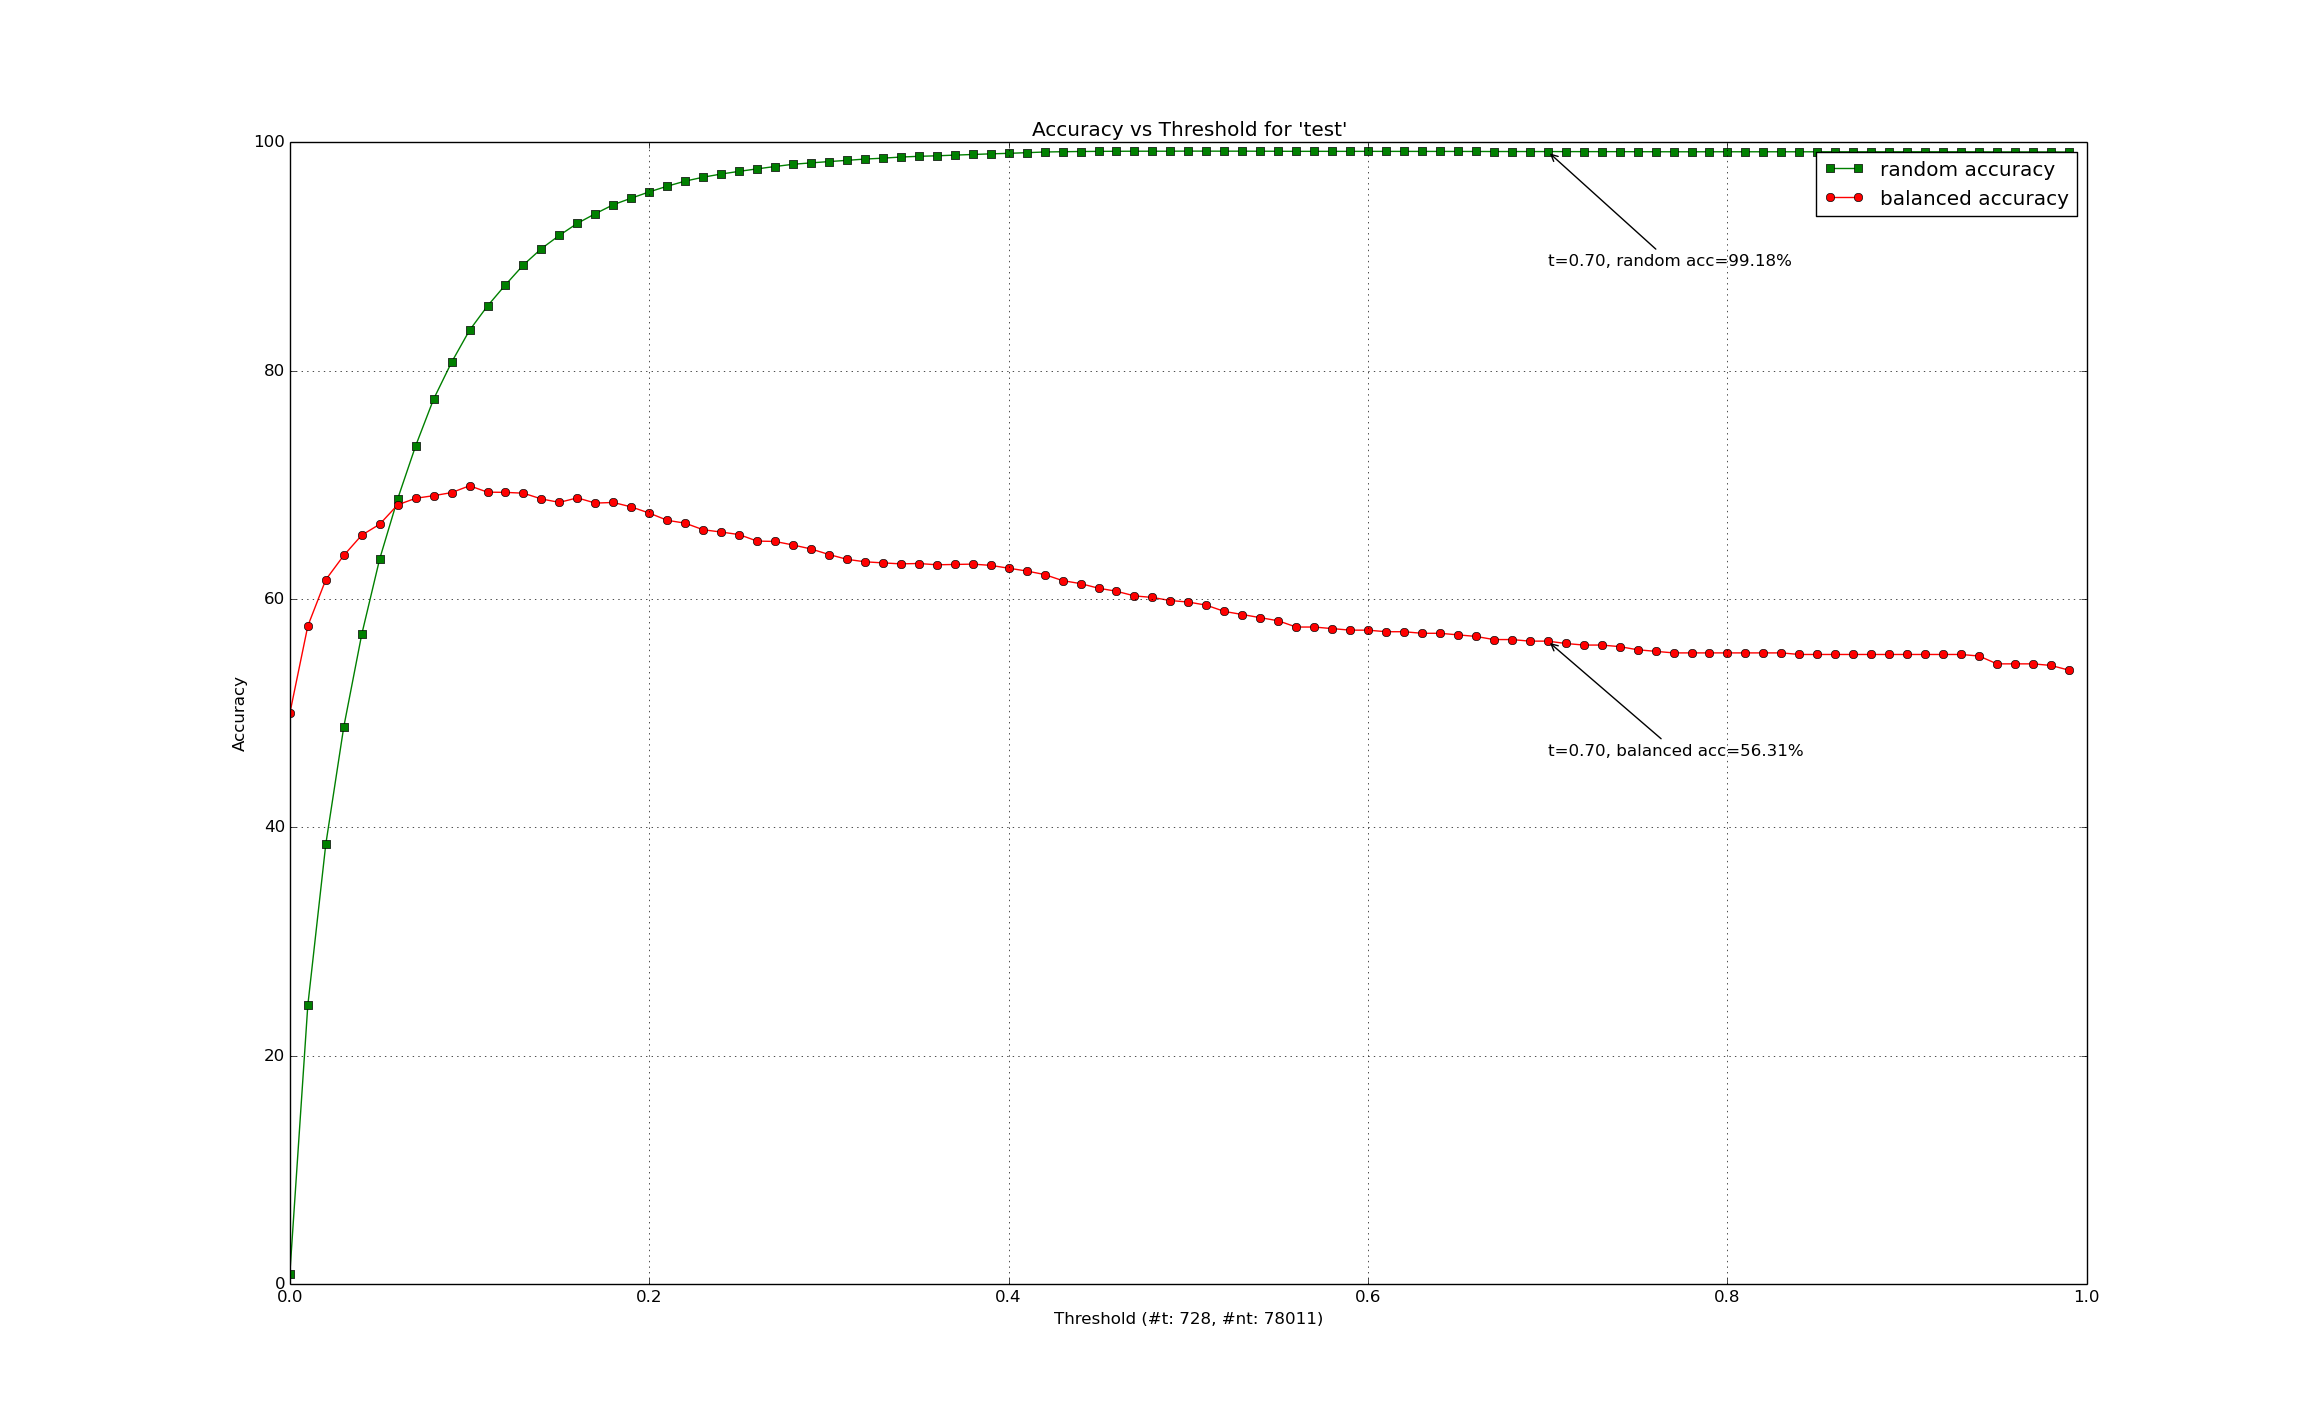
\includegraphics{images/test_accuracy_plot.png}\hfill}

The plot shows the random and the balanced accuracy for a range of threshold values.
In the plot the accuracy at the system's decision threshold is indicated. H.L. the treshold was set to 0.70.
This value obviously depends on the system under test. The number of target tests (\#t) and the number of non target tests (\#nt) is shown in the x-axis label.
The threshold value can be set via the command line option `-d' or the `threshold' option.

\begin{Verbatim}[commandchars=\\\{\}]
                          number of true positives + number of true negatives
random accuracy= -----------------------------------------------------------------------------
                 number of true positives + false positives + false negatives + true negatives


                    sensitivity + specificity        0.5 * true positives                   0.5 * true negatives
balanced accuracy = -------------------------- = --------------------------------  +  ----------------------------------
                                2                true positives + false negatives      true negatives + false positives
\end{Verbatim}


\chapter{EER plot}
\label{eerplot:eer-plot}\label{eerplot::doc}\label{eerplot:eerplot-label}
Will plot a cumulative score plot showing the odds of a false positive and false negative
versus the raw scores. In order to draw the curves, the number of scores equal to or bigger than
a threshold are counted. This is done for a number of threshold values. The number can be set via
nrSamples4Probability in bioplot.cgf in section {[}probability{]}. The default is 250 steps.

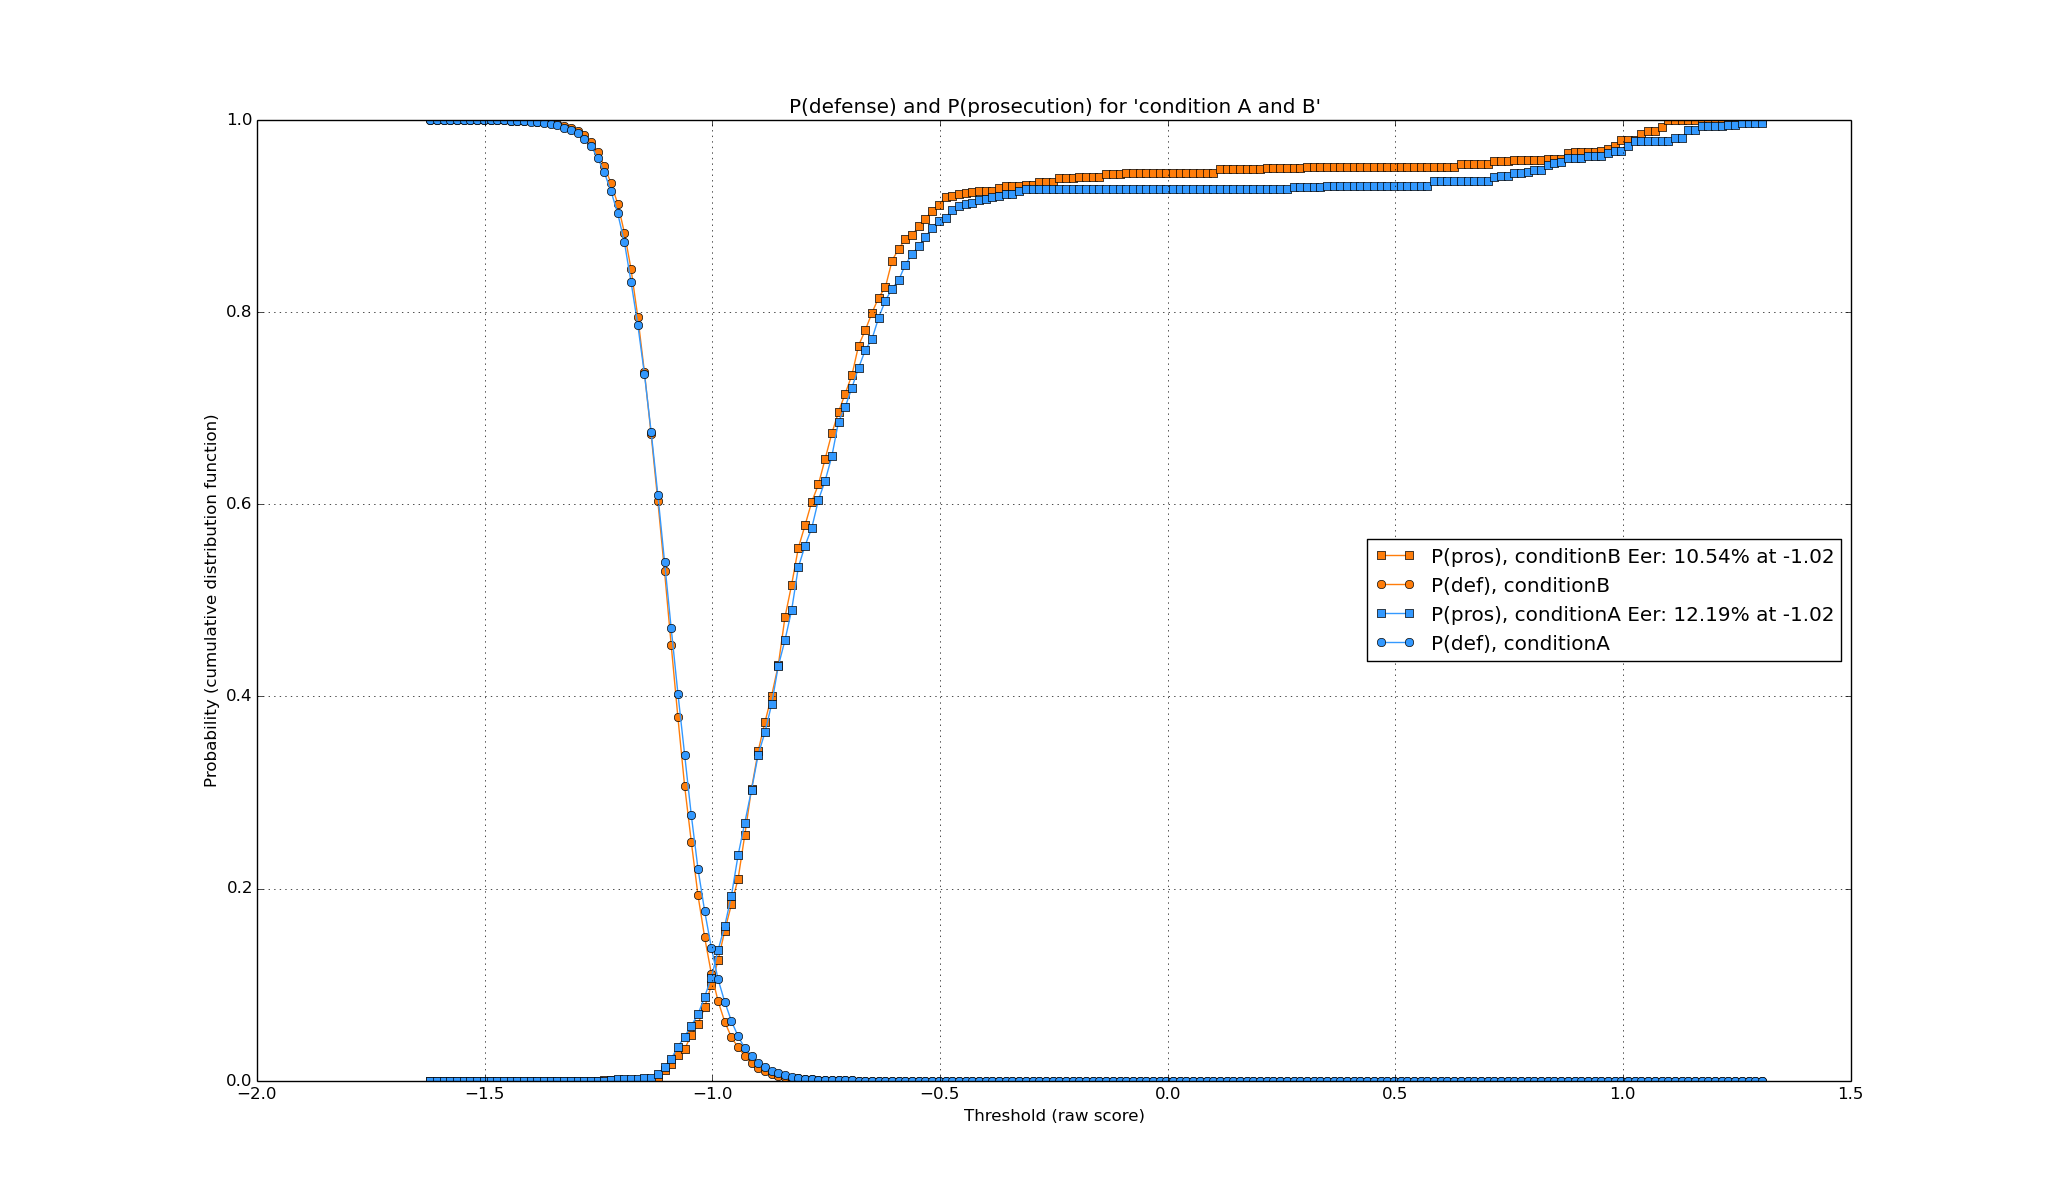
\includegraphics{images/condition_A_and_B_eer_plot.png}

ALl plots are shown in a window that allows you to zoom in on events. Here the plot is zoomed in around the intersection points of the graphs.

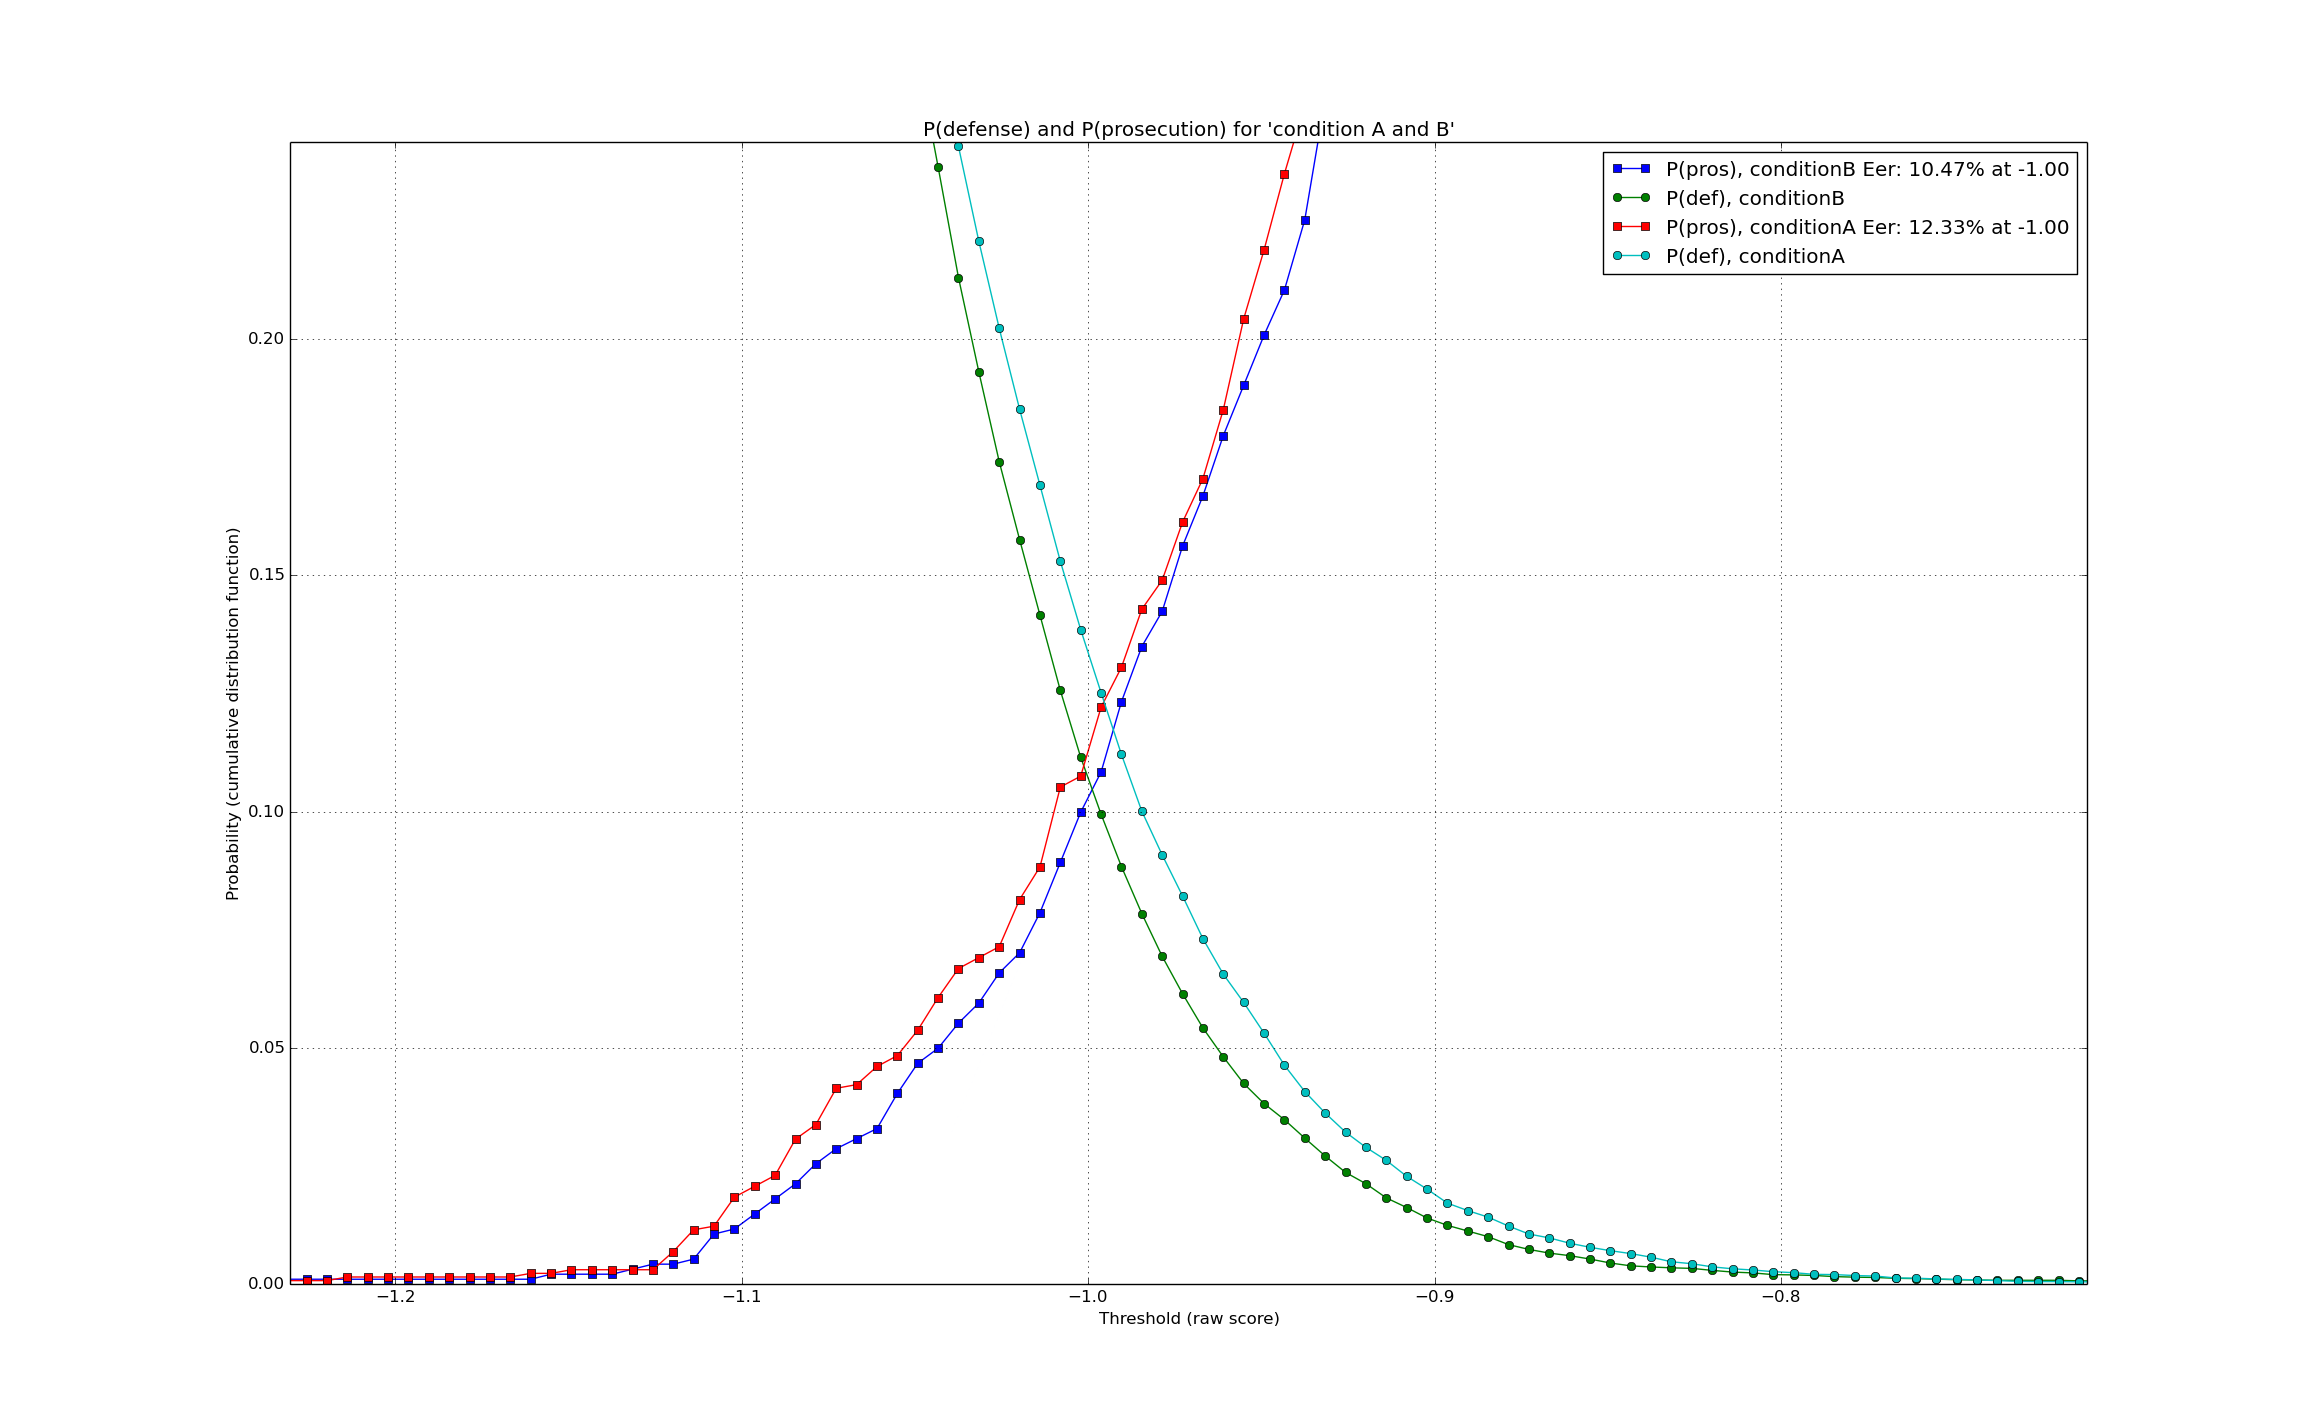
\includegraphics{images/condition_A_and_B_eer_plot_zoom.png}


\chapter{Histogram}
\label{histogram::doc}\label{histogram:histogram}
Nothing much to say about histograms. Here is an example:

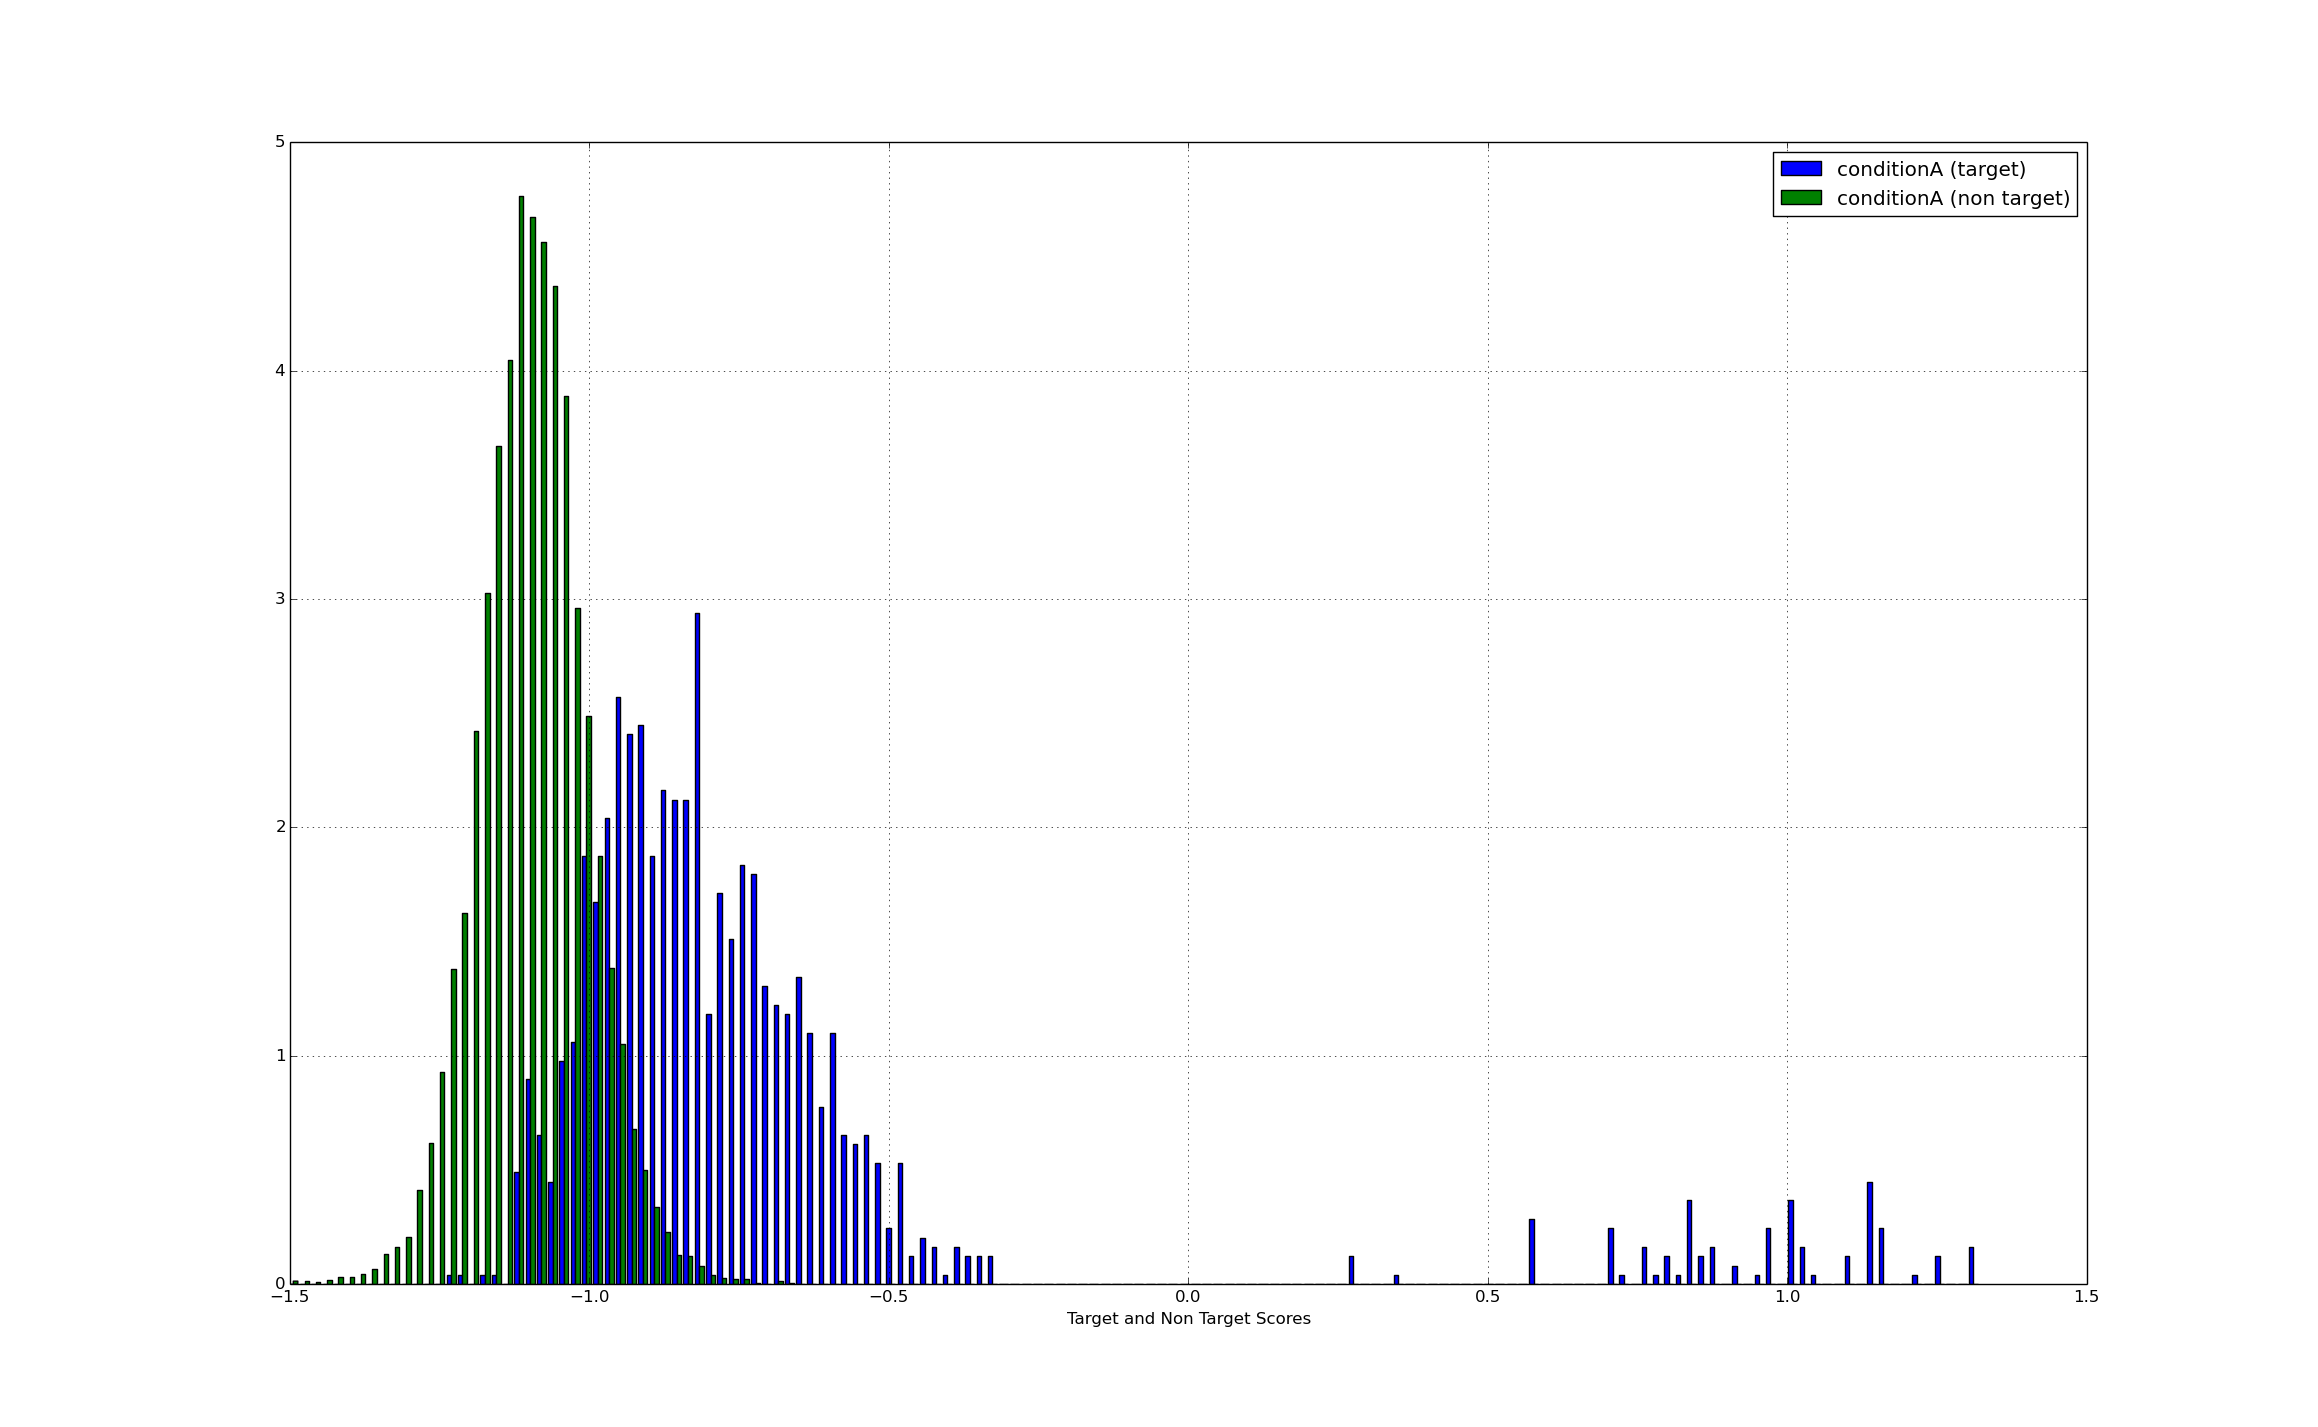
\includegraphics{images/condition_A_histogram_plot.png}

You can set the  number of bins used in bioplot.cfg:

\begin{Verbatim}[commandchars=\\\{\}]
\PYG{p}{[}\PYG{n}{histogram}\PYG{p}{]}
\PYG{n}{nrBins} \PYG{o}{=} \PYG{l+m+mi}{150}
\end{Verbatim}

The window showing the plot allows one to zoom in as shown in this example:

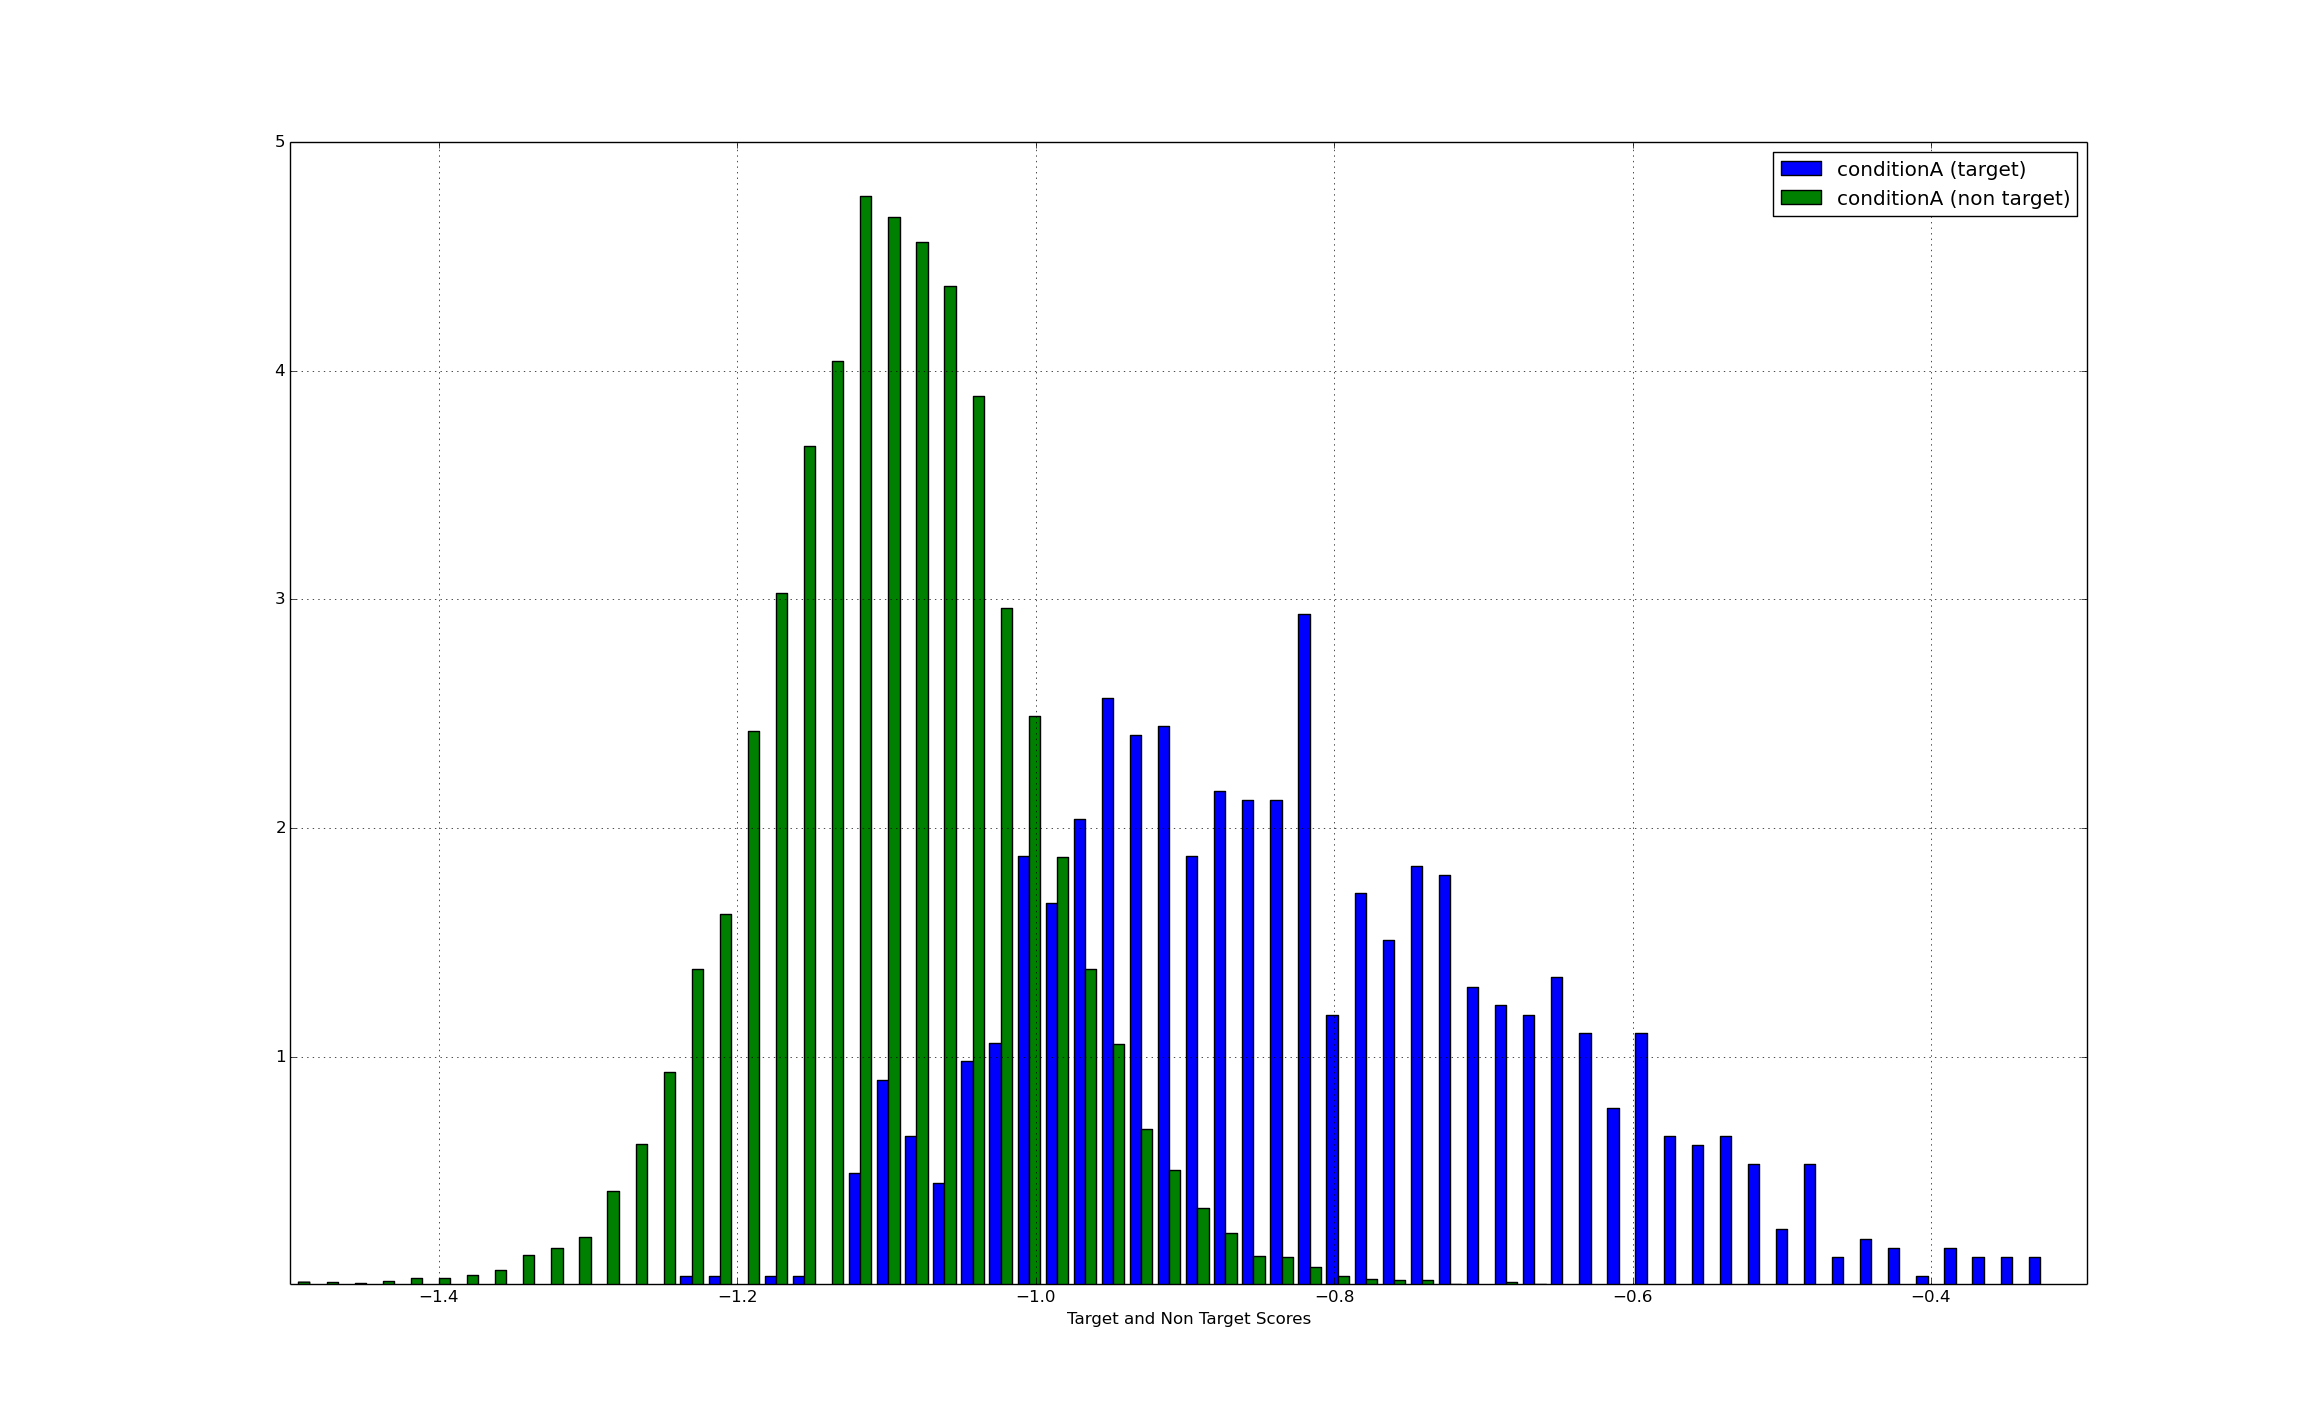
\includegraphics{images/condition_A_histogram_plot_detail.png}

Bioplot can produce cumulative plots as well. But they do not look very nice.
Have a look at {\hyperref[eerplot:eerplot-label]{\emph{EER plot}}}, this looks much nicer and in fact shows the same information.

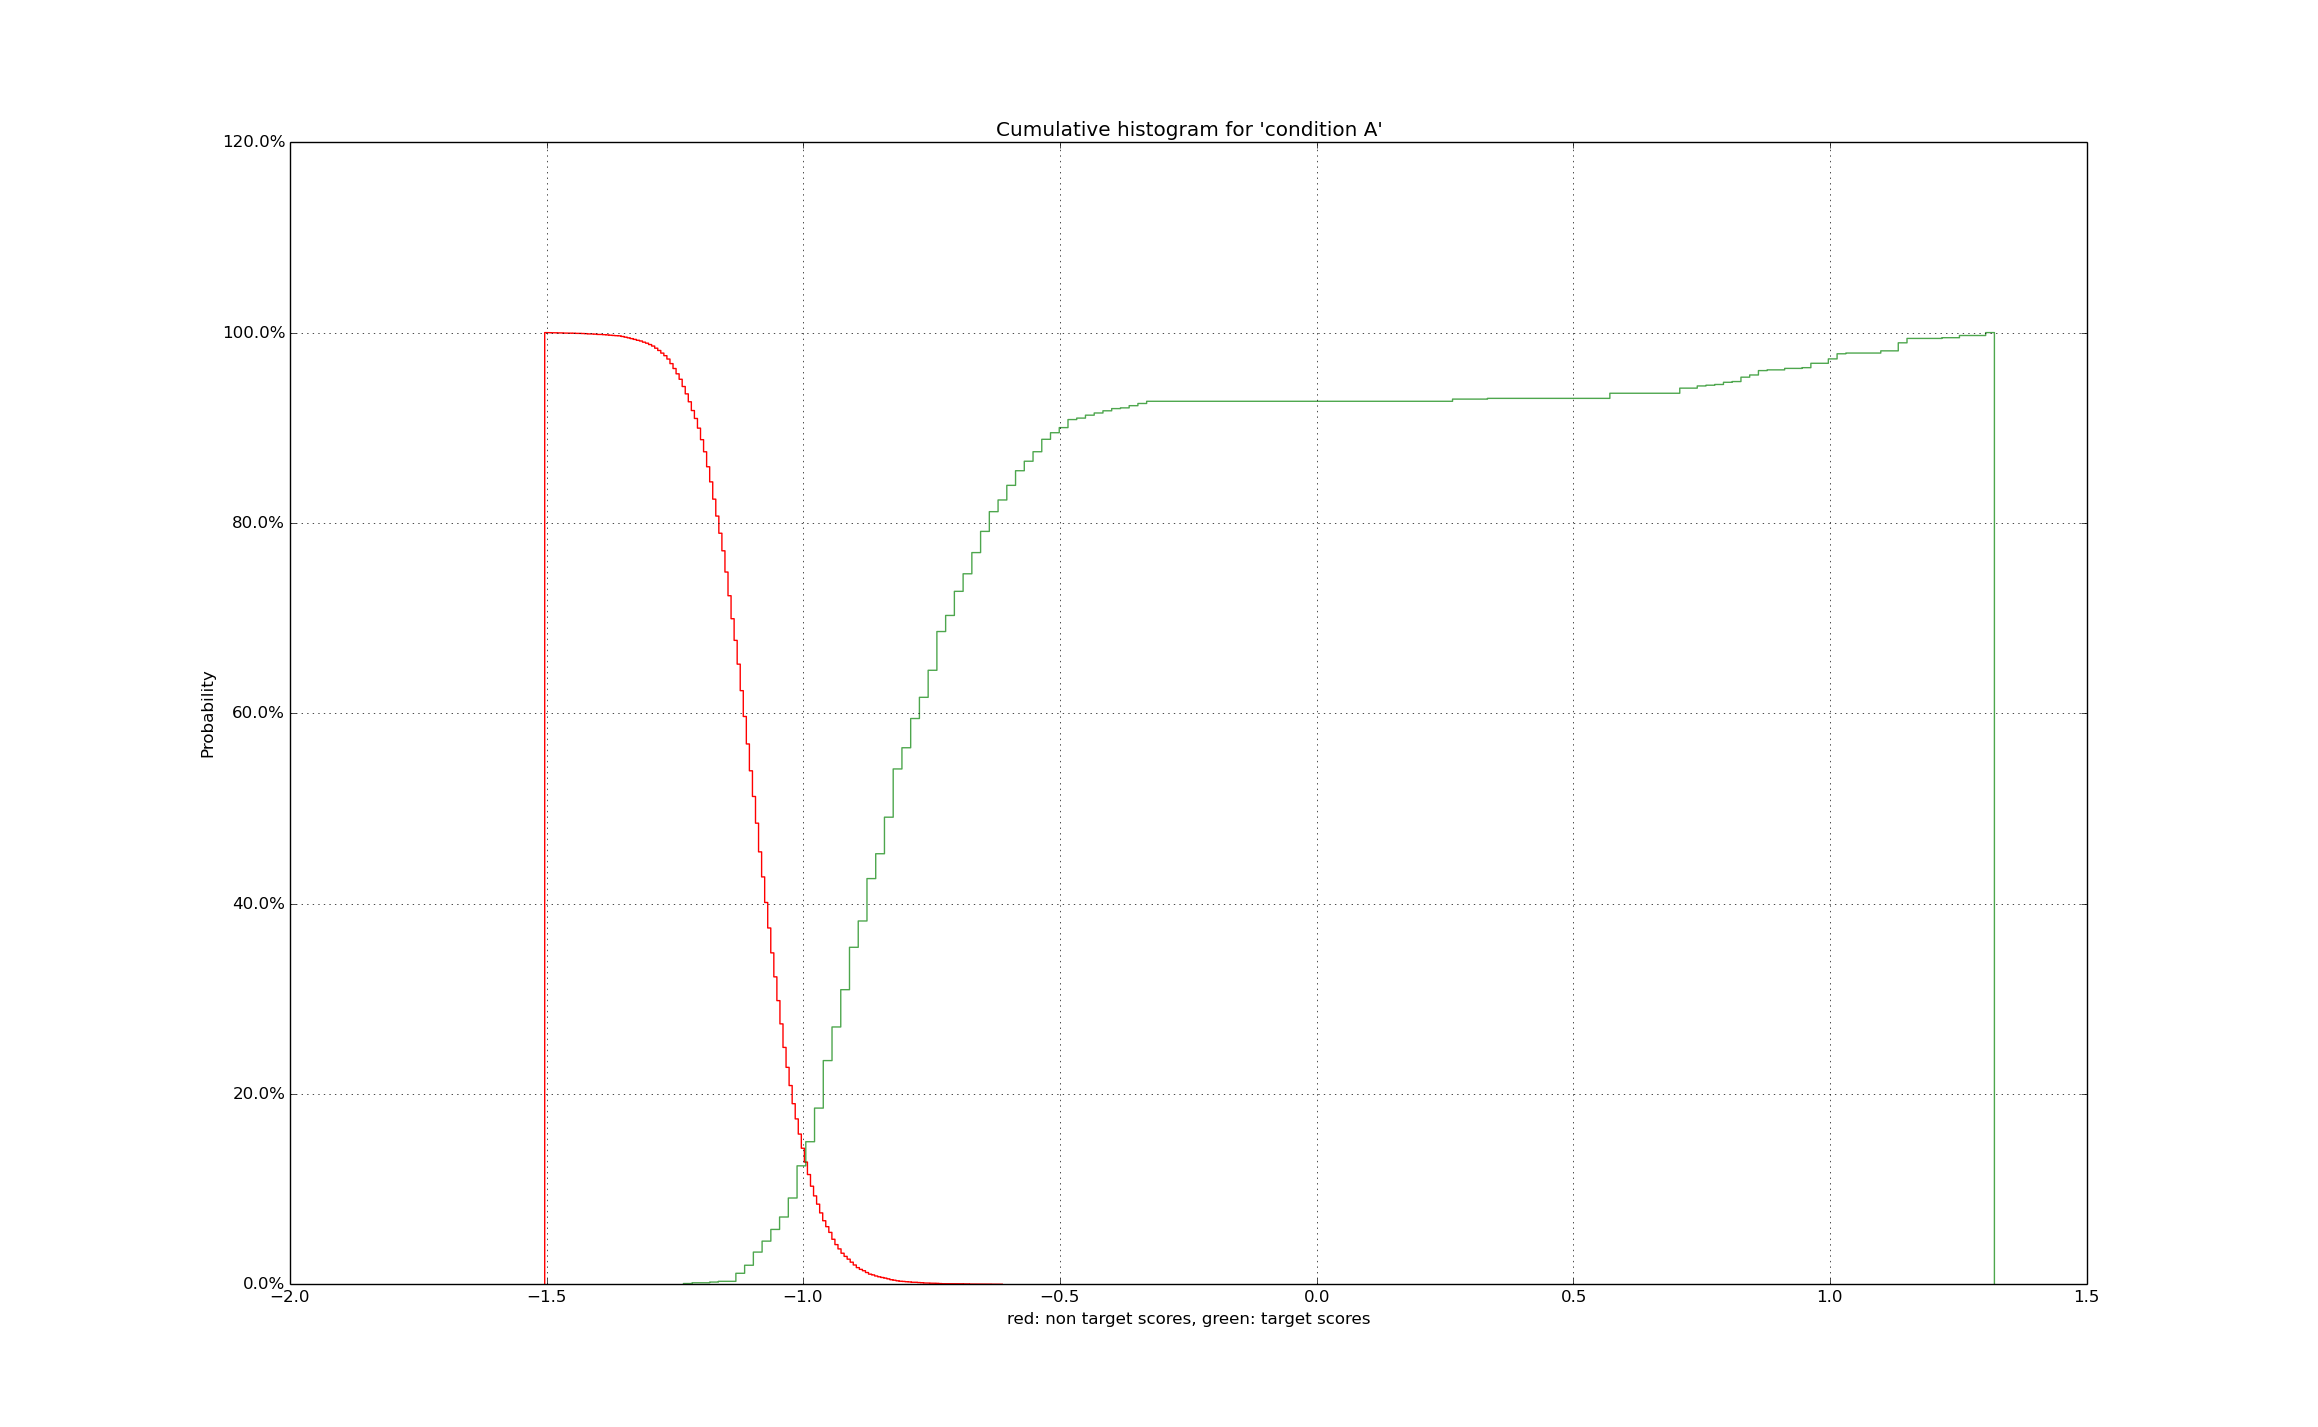
\includegraphics{images/condition_A_cumulative_histogram_plot.png}


\chapter{Matrixplot}
\label{matrixplot:matrixplot}\label{matrixplot::doc}
A matrix plot can be used to compare scores of different experiments with eachother. It is also usefull to display correlations. If the scores contain labels compared to other labels each comparison resulting in one score, then the plot will show a correlation plot. If labels are compared to multiple instances of other labels, each resulting in groups of scores, then these groups are averages.
To differentiate between experiments the meta value field of the data file is used.

Matrices can be combined in one plot. Example:

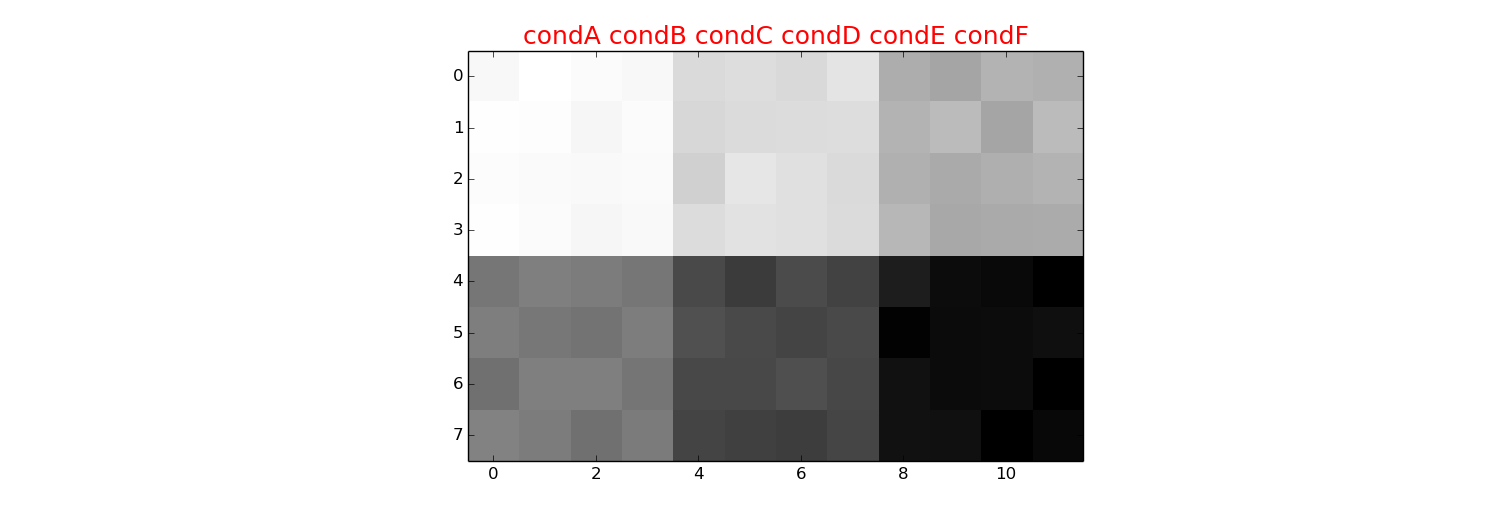
\includegraphics{images/matrix_data_6conditions.png}

This plot shows 6 conditions where the overall score changes from condition to condition. The first 3 labels
correspond to the top row of matrices (from left to right), the next 3 with the bottom row.
If the number of conditions allows it, the plots can be combined into one plot as in the example above.
But it is possible to plot them all next to eachother or above oneanother. If the vertical dimension of each matrix exceeds the horizontal dimension they will be drawn next to each other, otherwise they will be drawn in a vertical bar. To achieve this, set combineMatrices to False in bioplot.cfg:

\begin{Verbatim}[commandchars=\\\{\}]
\PYG{p}{[}\PYG{n}{matrix}\PYG{p}{]}
\PYG{n}{combineMatrices} \PYG{o}{=} \PYG{n+nb+bp}{False}
\end{Verbatim}

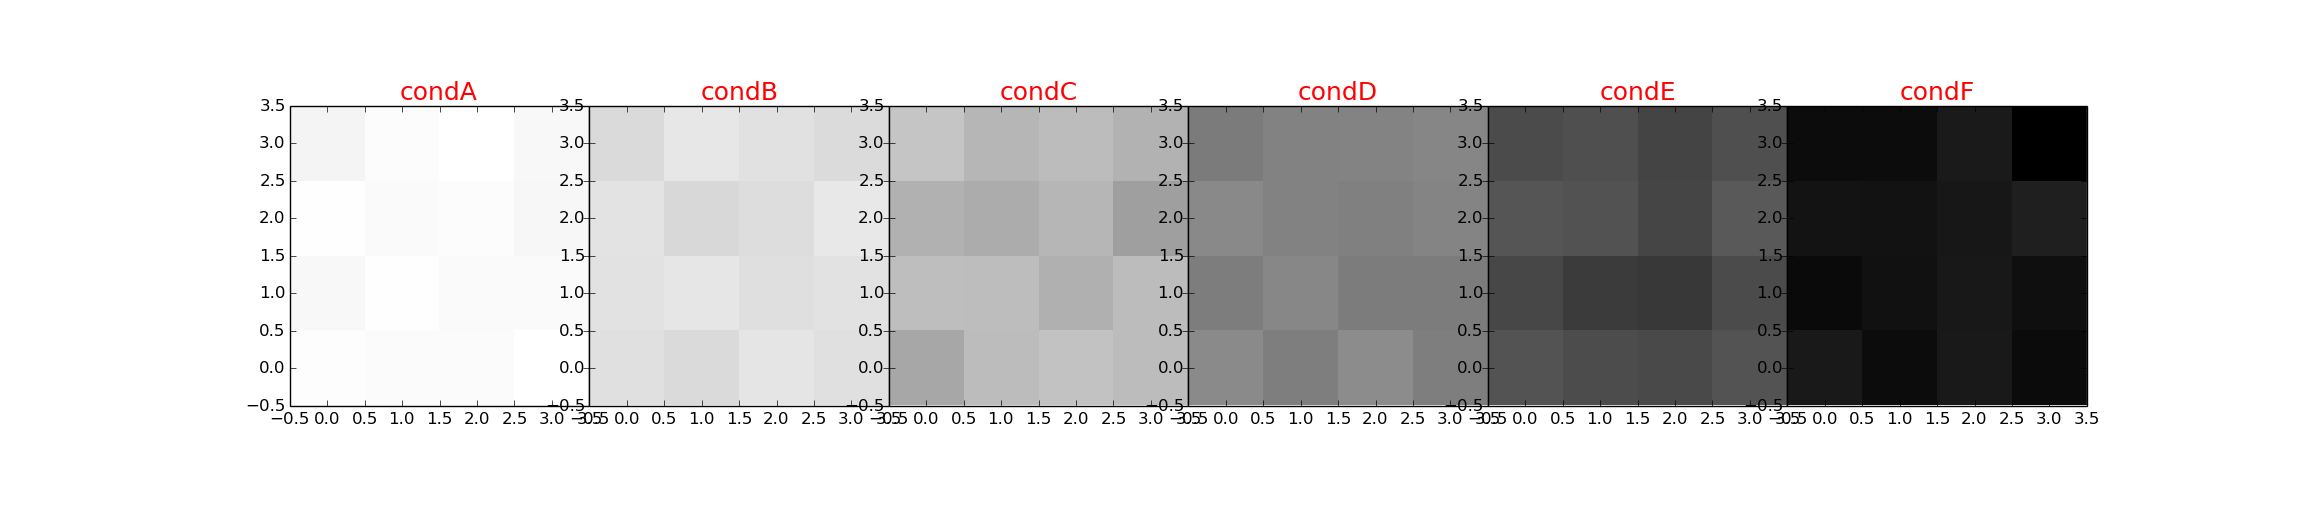
\includegraphics{images/matrix_data_horizontal_6conditions.png}

If you want to see some labels in the plot, add the following to bioplot.cfg:

\begin{Verbatim}[commandchars=\\\{\}]
\PYG{p}{[}\PYG{n}{matrix}\PYG{p}{]}
\PYG{n}{showLabels} \PYG{o}{=} \PYG{n+nb+bp}{True}
\PYG{n}{labelAngle} \PYG{o}{=} \PYG{l+m+mi}{70}
\end{Verbatim}

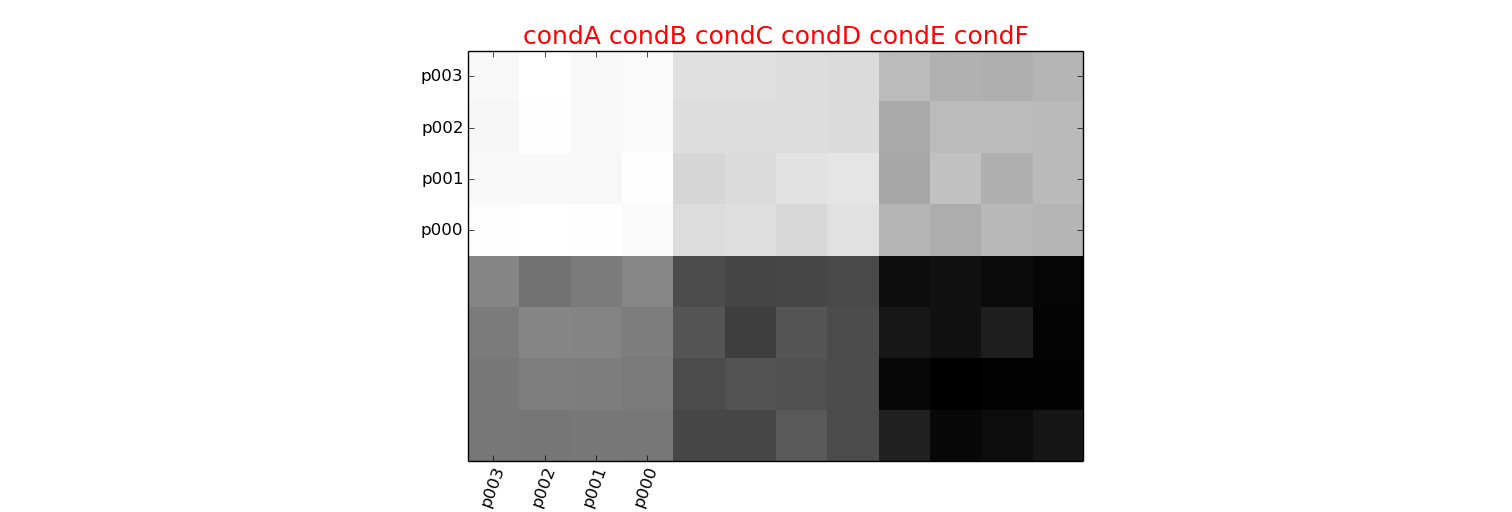
\includegraphics{images/matrix_data_6conditions_with_labels.png}

The matrices above contain artifical data. In real experiments not all labels may have the same number of scores. This may be due to data shortage, a model not being computed etc. In that case bioplot will accept the scores that exist and plot as many as possible. This is visible in the matrices below. On the right hand side data that is missing is replaced by some average value. The scaling of the grey values is not influenced by these values.

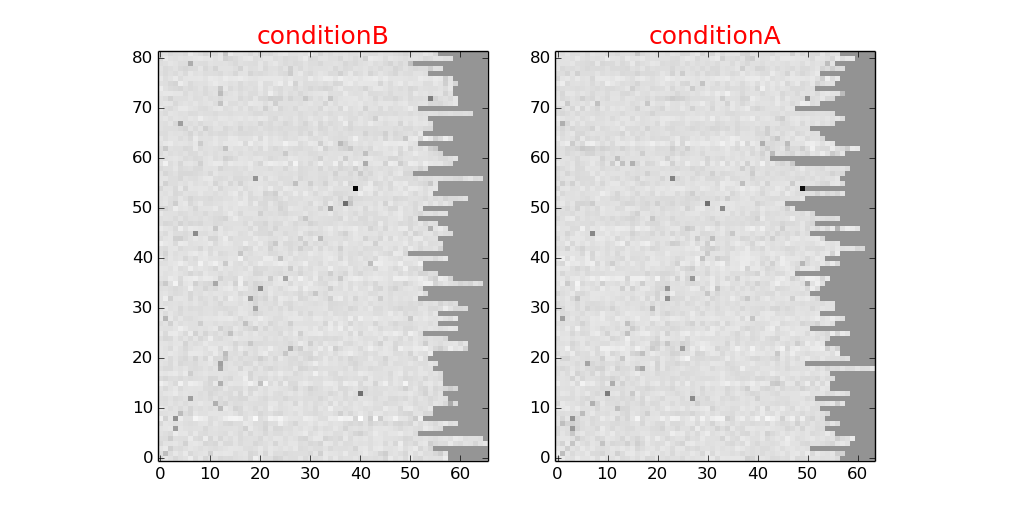
\includegraphics{images/real_data_matrix_plot.png}


\chapter{Ranking plot}
\label{rankingplot:ranking-plot}\label{rankingplot::doc}
Bioplot.py allows you to plot a ranking plot. Example run:

\begin{Verbatim}[commandchars=\\\{\}]
python ./bioplot.py -e 'A' -f testdata\_A.txt -R
\end{Verbatim}

E.g. if looking for a picture in a database a face recognition system may return a list of potential hits. This plot shows what the odds are that the target will be in the first N pictures.

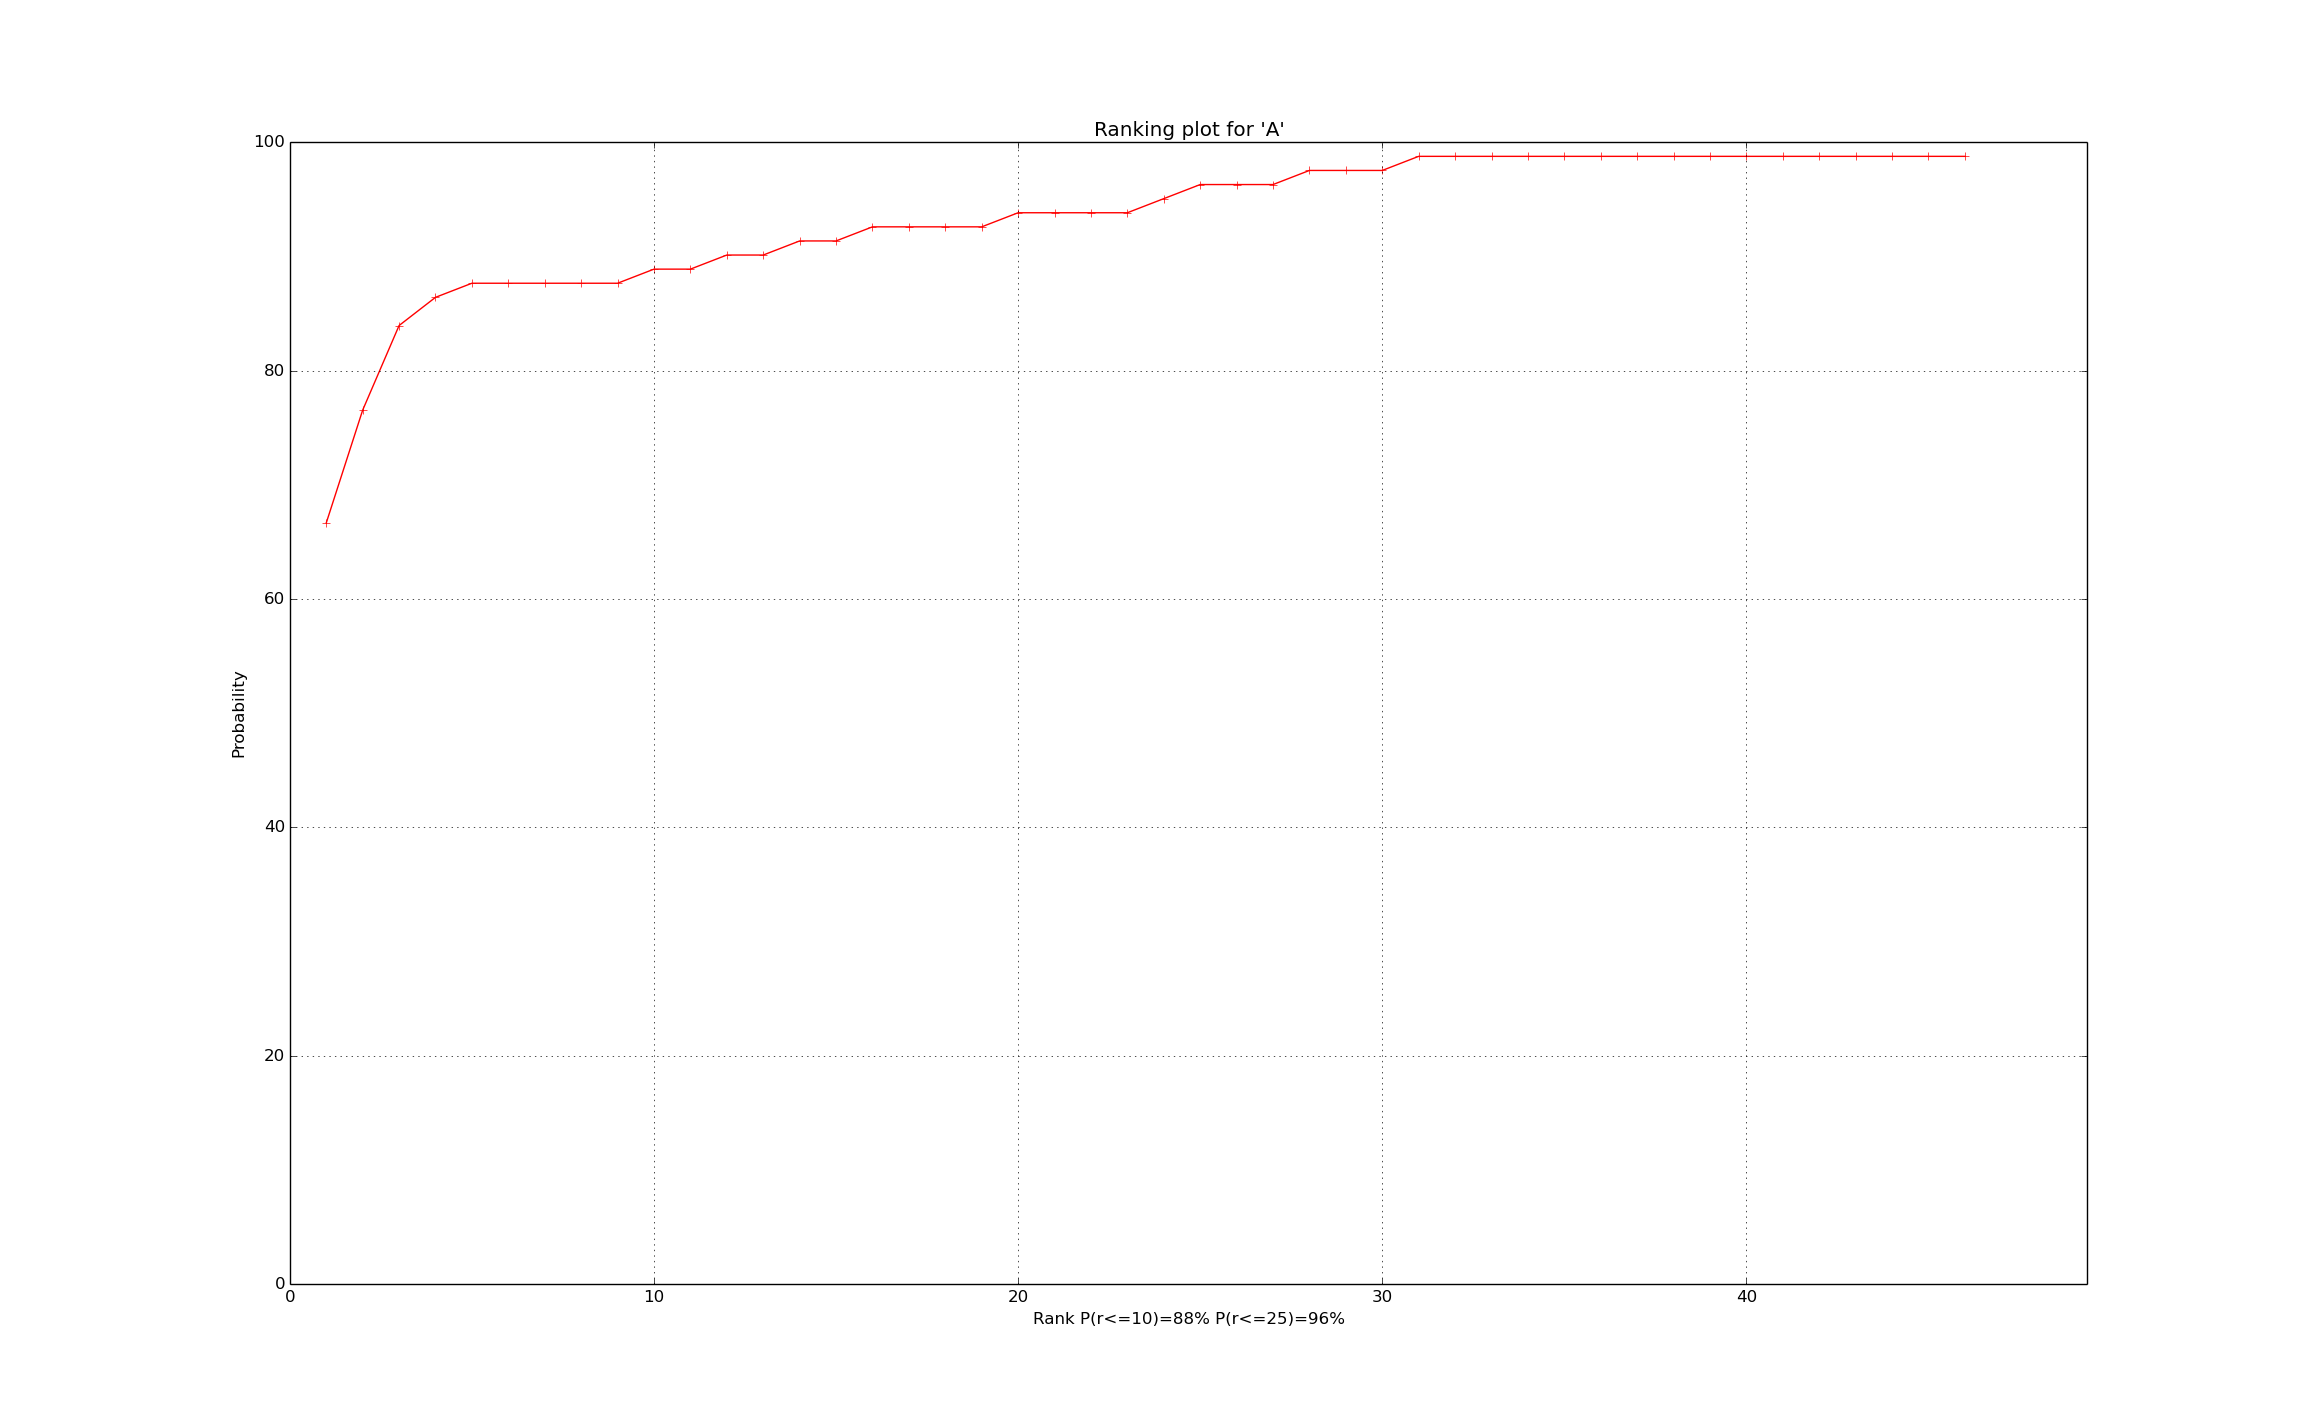
\includegraphics{images/A_ranking_plot.png}


\chapter{Tippett plot}
\label{tippettplot::doc}\label{tippettplot:tippett-plot}
Will plot a tippet plot showing the odds of a false positive and false negative
versus the raw scores. In order to draw the curves, the number of scores equal to or bigger than
a threshold are counted. This is done for a number of threshold values. The number can be set via
nrSamples4Probability in bioplot.cgf in section {[}probability{]}. The default is 250 steps.

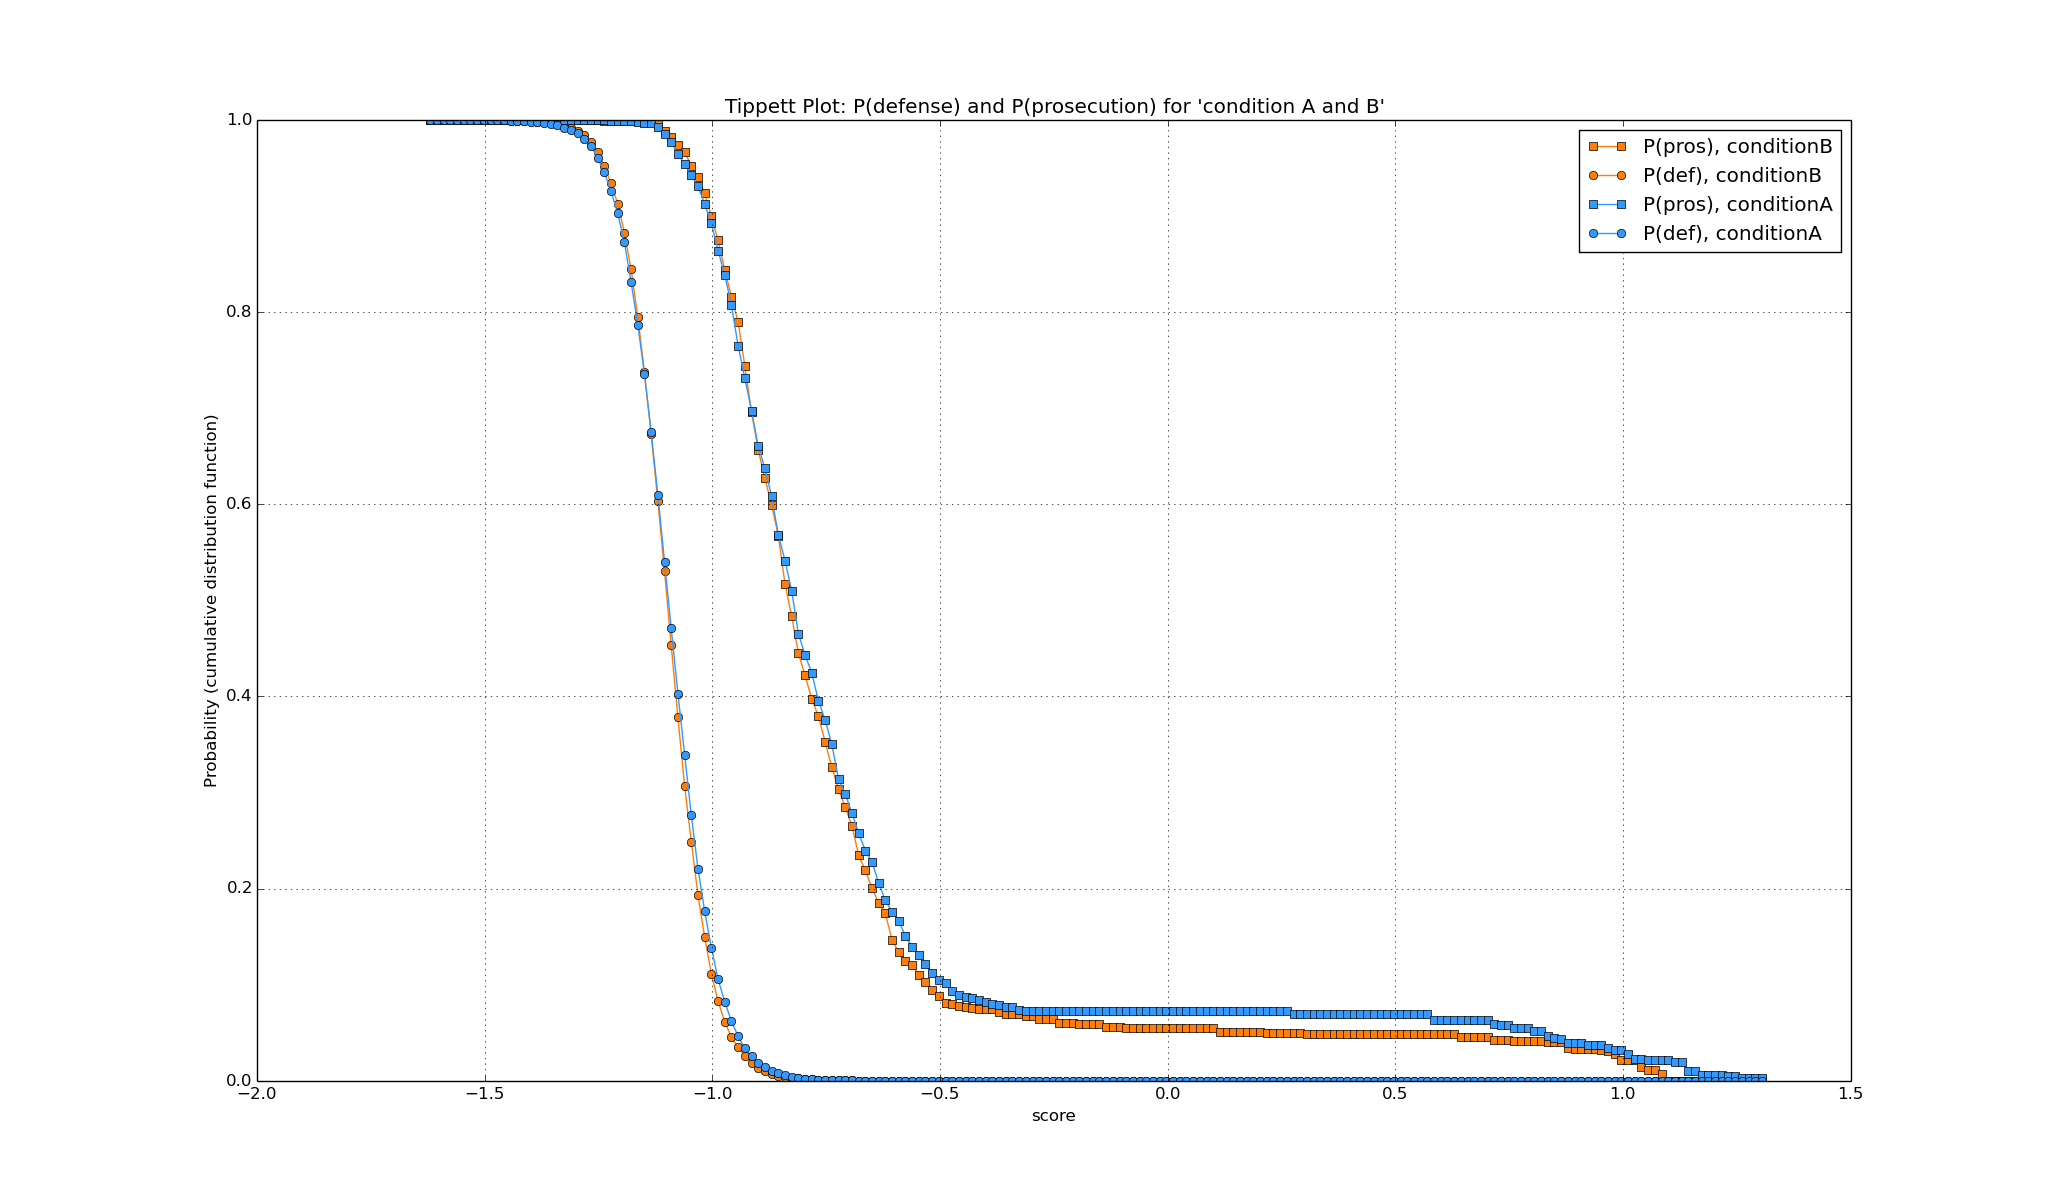
\includegraphics{images/condition_A_and_B_tippett_plot.png}


\chapter{Zoo plot}
\label{zooplot:zoo-plot}\label{zooplot::doc}\label{zooplot:rst-zooplot}
A zoo plot shows a scatter type plot where on the vertical axis the mean of the non target
scores and on the horizontal axis the mean target scores are drawn for each label. This leads to
a plot of dots where each dot represents one speaker ( assuming the data stems from a speaker
id experiment ).
The plot below shows combined data of 3 experiments (A, B and C). The legend shows the eer values for the respective conditions.
To get bioplot to show this legacy type zoo plot, set the following option in bioplot.cfg:

\begin{Verbatim}[commandchars=\\\{\}]
\PYG{p}{[}\PYG{n}{zoo}\PYG{p}{]}
\PYG{n}{alexanderStyle} \PYG{o}{=} \PYG{n+nb+bp}{False}
\end{Verbatim}

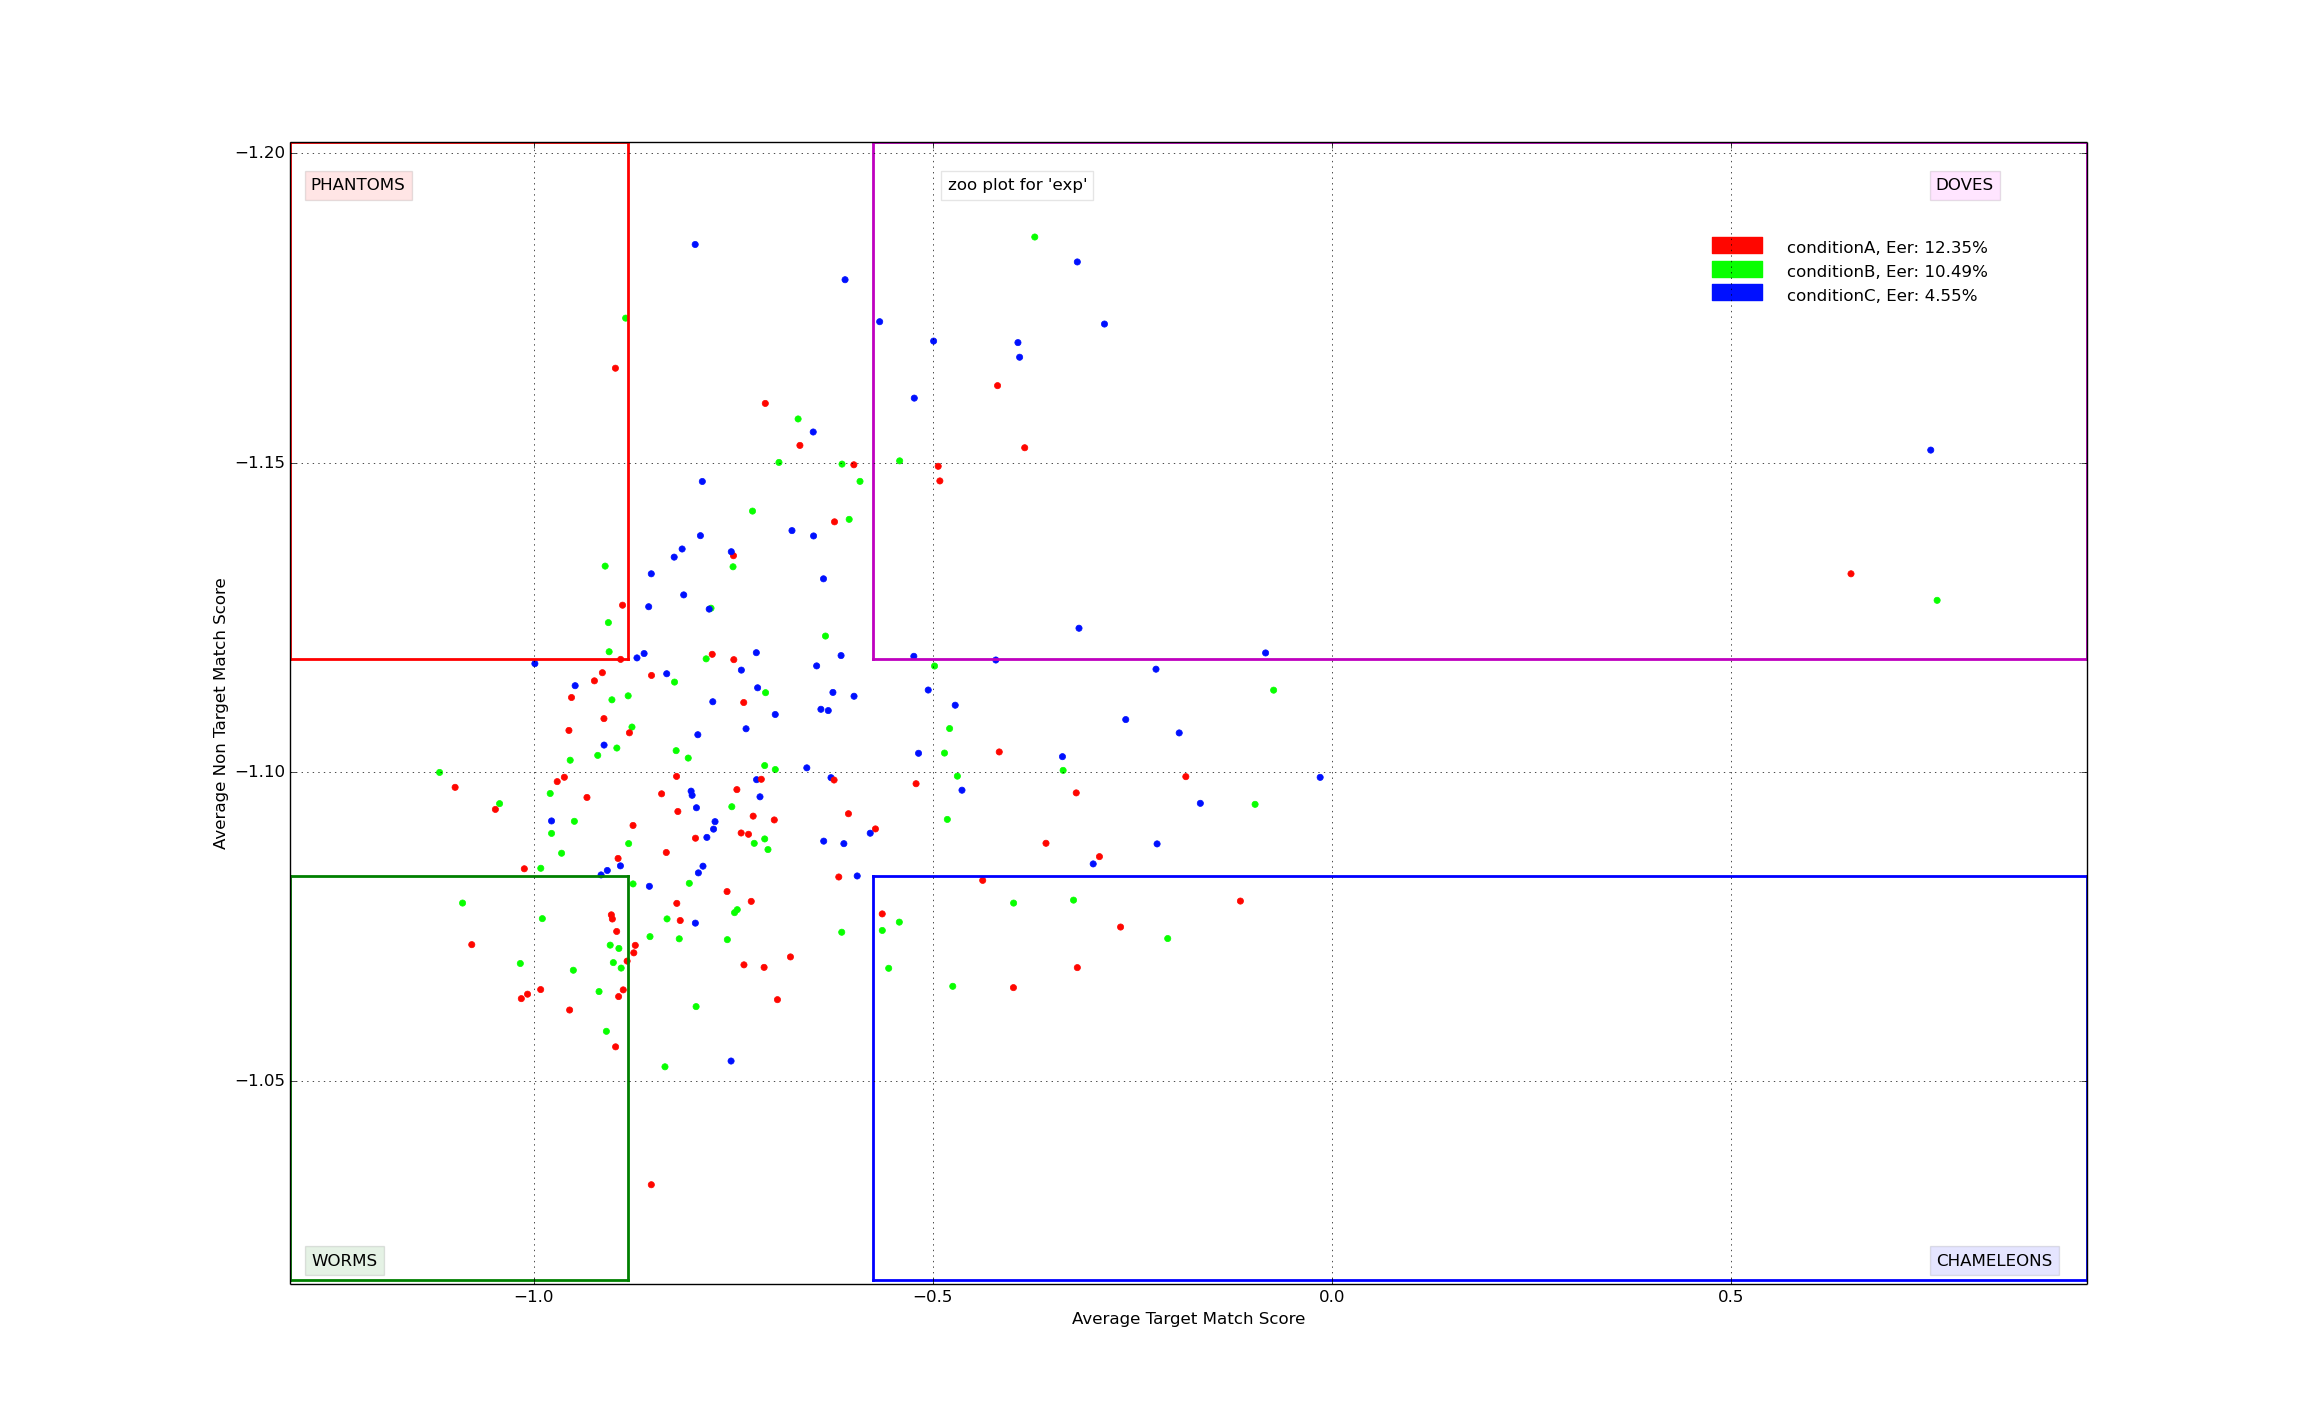
\includegraphics{images/exp_zoo_plot.png}

An extention of the zoo plots was shown at the IAFPA 2014 conference in Zurich, Switserland
by Anil Alexander et al. They proposed that adding a measure of the standard deviations of the
scores used to make the plot will add details of the score distributions of the persons
to the plot. If the option alexanderStyle in {[}zoo{]} is set to True, ellipses are drawn
at the positions where the points of a traditional zoo plot would be.
The width and height of the ellipses shown are essentially the standard deviations of the average
target and average non target scores for a given label. Because these may be much bigger or much
smaller than the horizontal and vertical scales of the traditional zoo plot, the mean standard
deviations are scaled by subtracting the overall mean standard deviation and dividing by the
standard deviation of all standard deviations. This is in essence a normalization procedure.
The result will be ellipses with a unit width and height and ellipses smaller and bigger than that.
To be able to actually plot the normalised ellipses, the width is multiplied by the range of
scores on the horizontal axis and the height is multiplied by the range of the scores on the vertical axis.
Finally to scale the ellipses their width and height is divided by a scale factor.
This scale factor is related to the number of pixels in the display used to plot the zoo plot.
A value of 150 works nicely for a 1600 ... 1280x1024 display.

To get bioplot to show this legacy type zoo plot, set the following option in bioplot.cfg:

\begin{Verbatim}[commandchars=\\\{\}]
\PYG{p}{[}\PYG{n}{zoo}\PYG{p}{]}
\PYG{n}{alexanderStyle} \PYG{o}{=} \PYG{n+nb+bp}{True}
\end{Verbatim}

If you don't like the colors used, choose a different value for colorMap from this list:
Spectral, gist\_ncar, hsv, gist\_rainbow or prism and set colorMap in bioplot.cfg:

\begin{Verbatim}[commandchars=\\\{\}]
\PYG{p}{[}\PYG{n}{cfg}\PYG{p}{]}
\PYG{n}{colorMap} \PYG{o}{=} \PYG{n}{hsv}
\end{Verbatim}

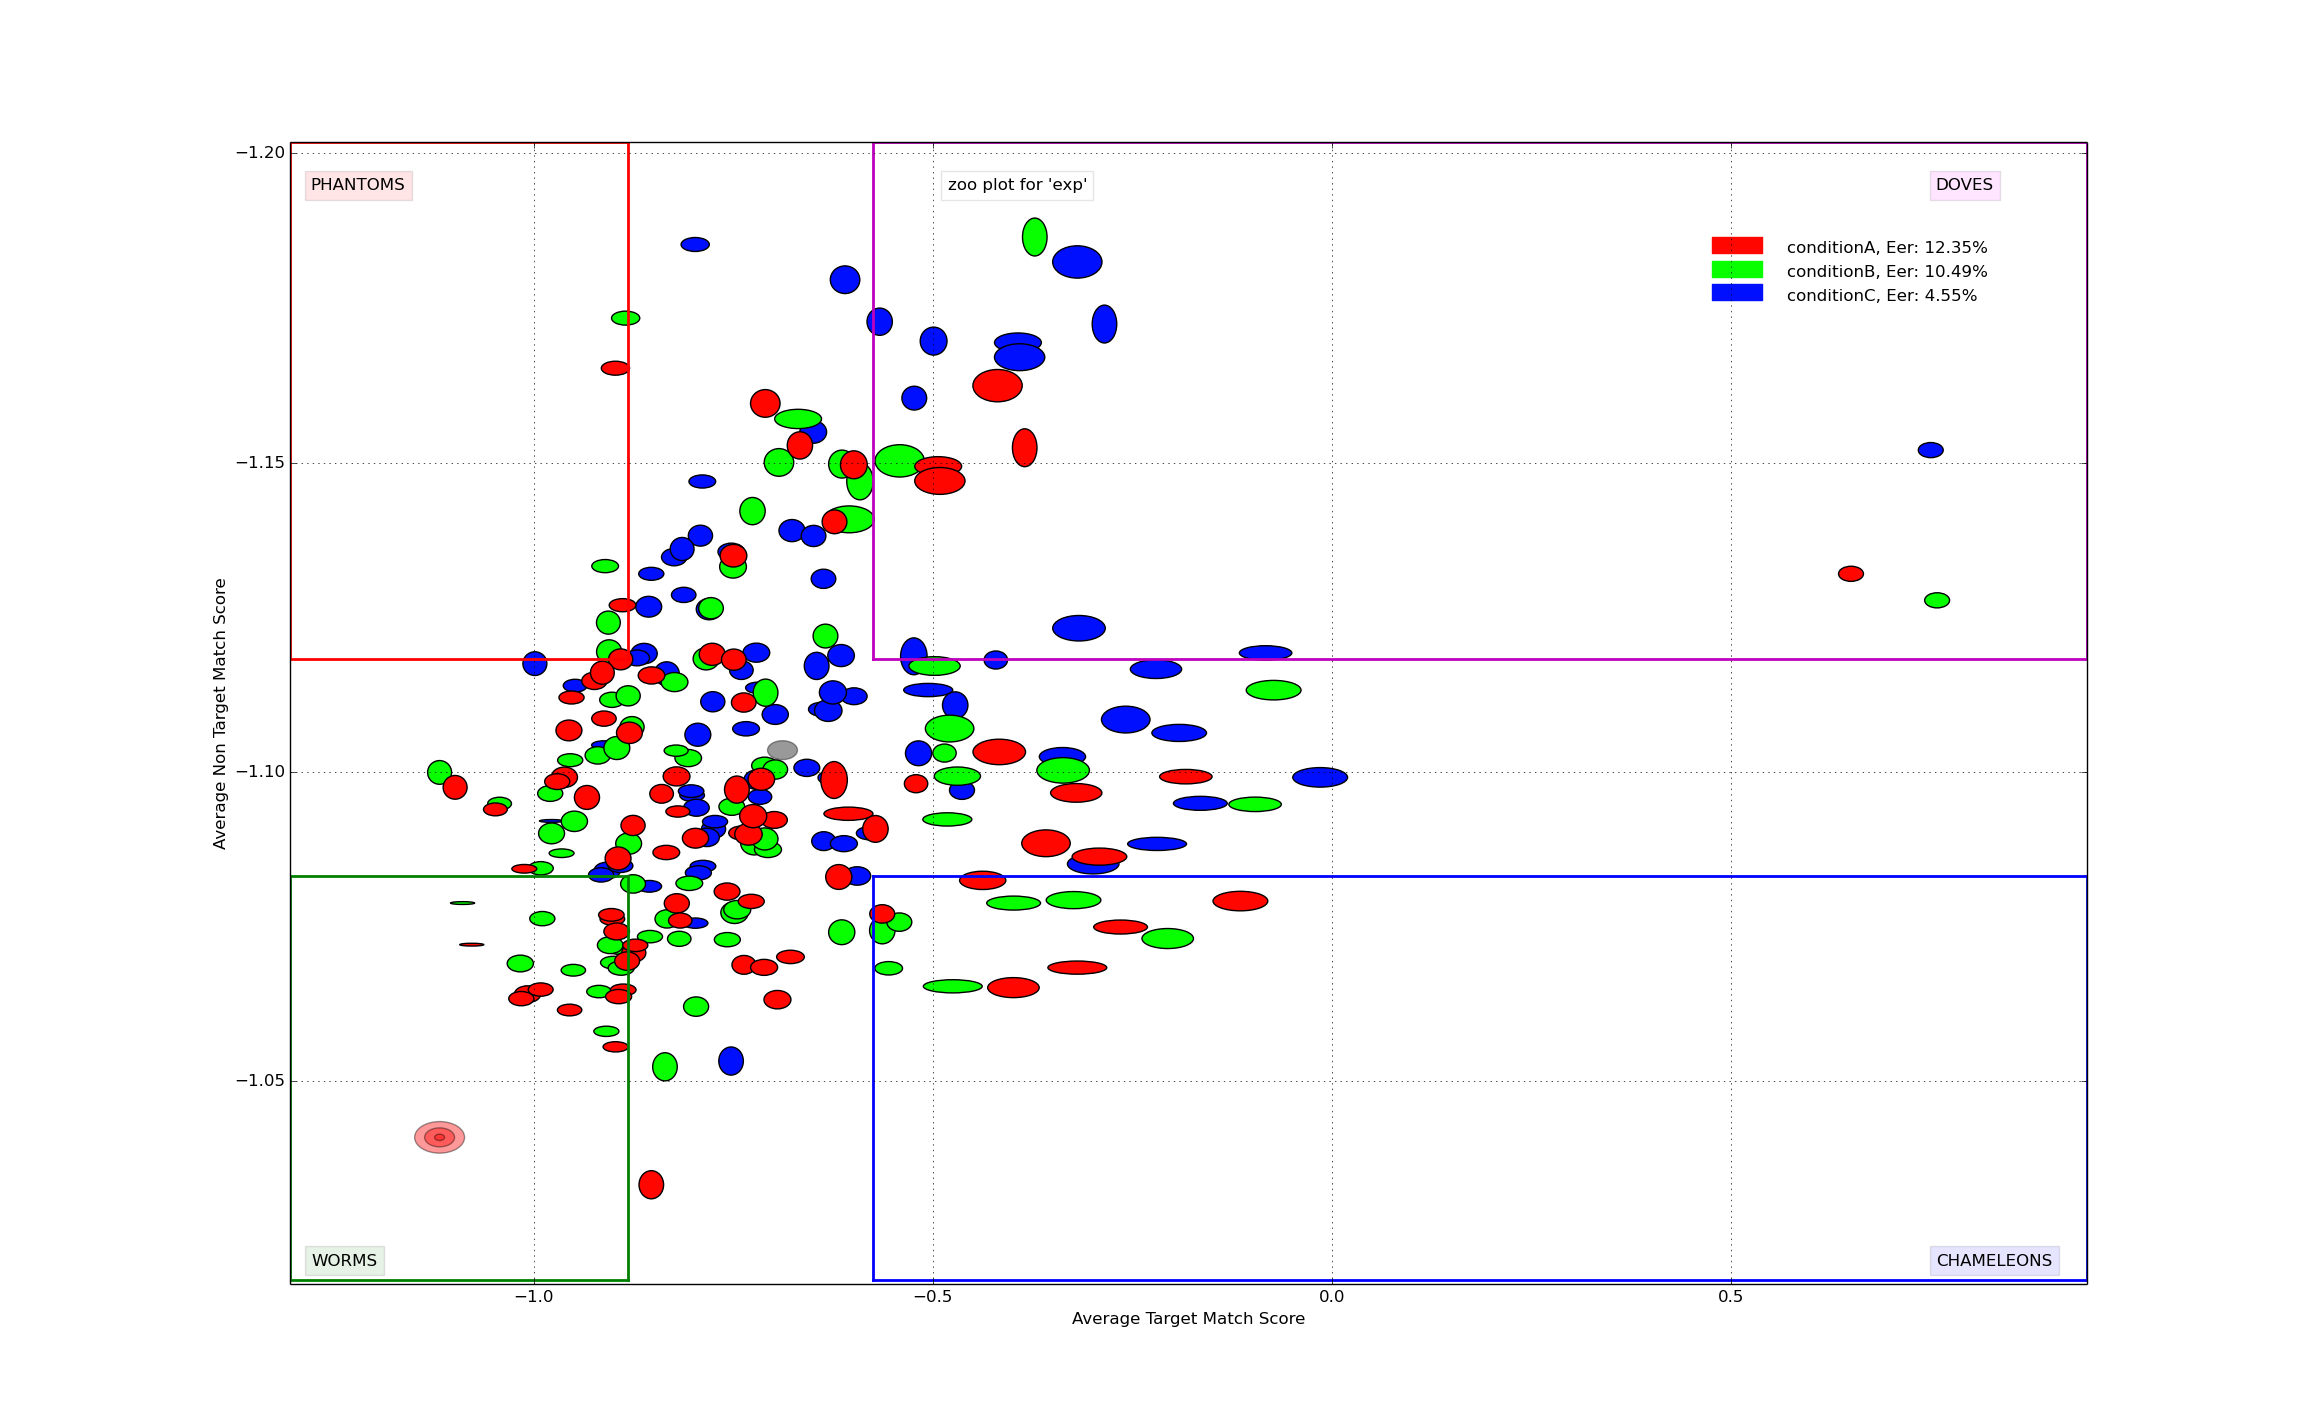
\includegraphics{images/exp_zoo_plot_01.png}

Note that the shape of the ellipses is influenced by the difference in range of the vertical and
horizontal axis. This means that comparing shapes between zoo plots with varying ranges of
mean target and mean non target scores can be very tricky.

The grey/black ellipse in the center of the quartiles denotes the mean of all ellipses. The 3 red ellipses on the lower
left are meant as reference points. Their sizes measure (from smallest to largest ellipse): mean - 2 standard deviations, mean, mean + 2 standard deviations. If you do not want these in your plot make the following setting:

\begin{Verbatim}[commandchars=\\\{\}]
\PYG{p}{[}\PYG{n}{zoo}\PYG{p}{]}
\PYG{n}{showReference} \PYG{o}{=} \PYG{n+nb+bp}{False}
\PYG{n}{showUnitDataPoint} \PYG{o}{=} \PYG{n+nb+bp}{False}
\end{Verbatim}


\section{Highlighting labels}
\label{zooplot:highlighting-labels}
If you click on a data point in the plot, a text label will be shown near the point. This makes
it possible to find the name of a data point in e.g. the quartile ranges.

If you are curious where the scores of a specific label are in the zoo plot, you need
not click on all of them to find it. You can specify the labels on the command line.
If they are in the plot, they will be highlighted. Example:

\begin{Verbatim}[commandchars=\\\{\}]
python ./bioplot.py -e "condition A and B" -f testdata\_AB.txt -Z 1100 1131 1042
\end{Verbatim}

This will highlight label 1100, 1131 and 1042 in the zoo plot compiled from
the data in `testdata\_AB.txt' and dim the colors of the other points in the plot
making it easy to create a picture for a publication or report. Text labels
will be displayed near the points selected.

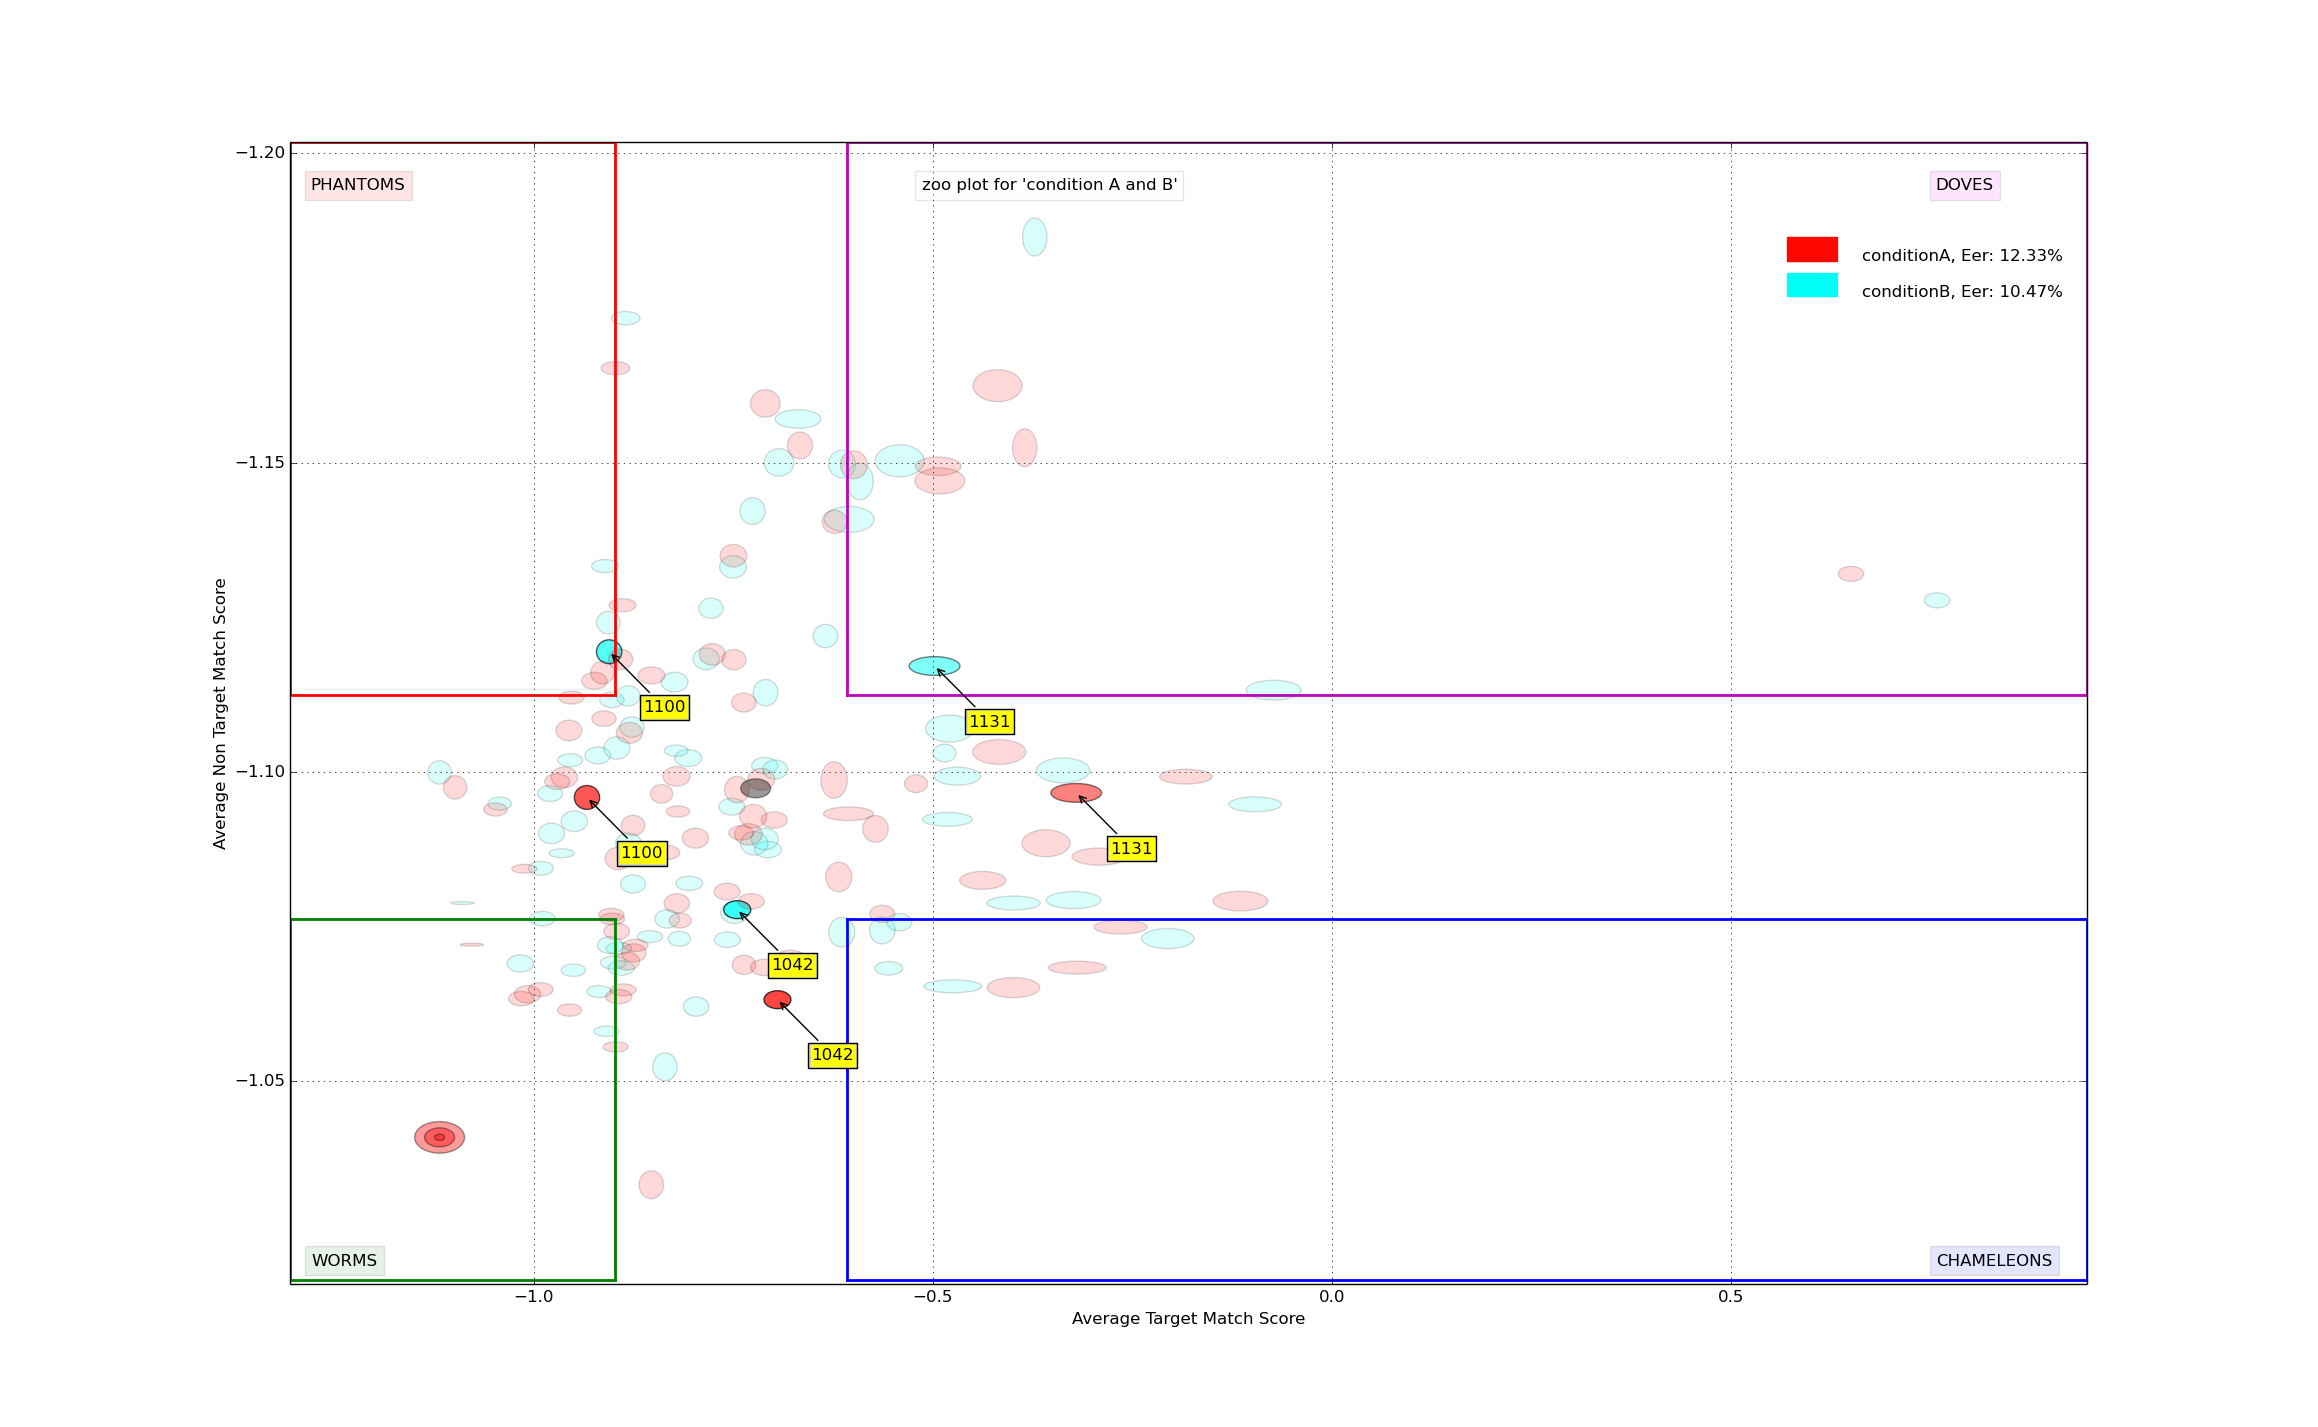
\includegraphics{images/condition_A_and_B_zoo_plot.png}

The lines between the ellipses connect labels which are equal. This makes
it easy to see what the effect of the parameter change is. Set interconnectMetaValues = True
in bioplot.cfg to acchieve this.

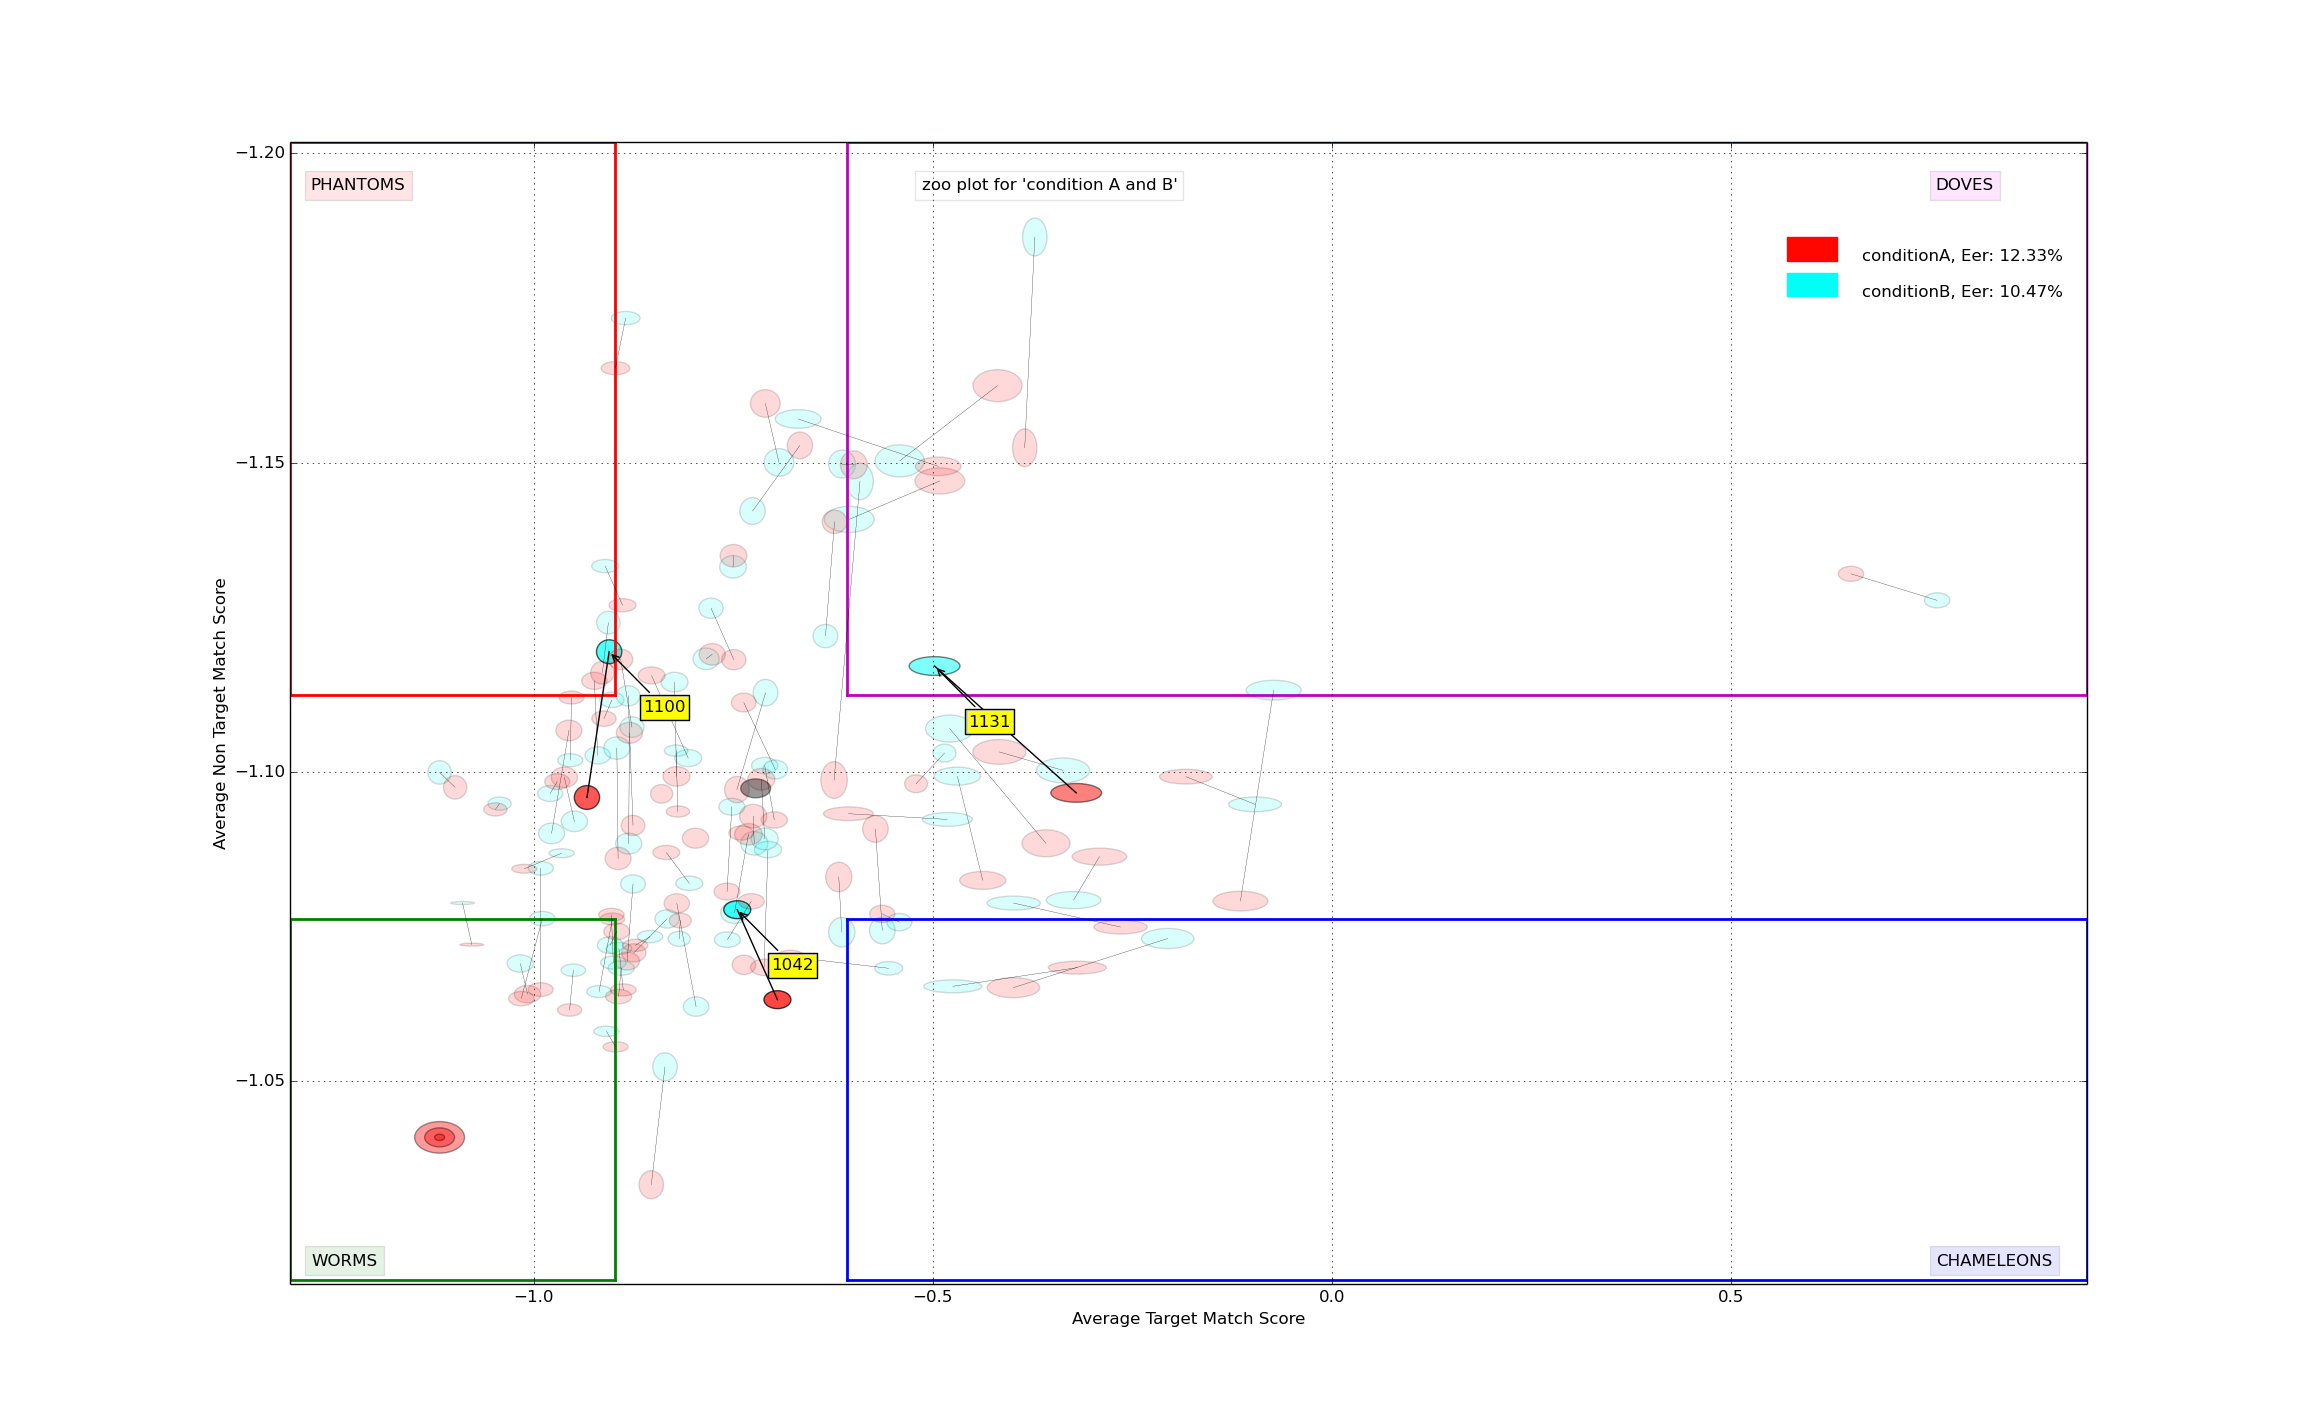
\includegraphics{images/condition_A_and_B_zoo_plot_01.png}


\section{Zooplots combined with Histograms}
\label{zooplot:zooplots-combined-with-histograms}
In the plot shown below the zoo plot is bordered by histograms showing the distributions of the target and non target scores. In this zoo plot 2 data sets are shown combined. The points corresponding with one label are interconneted. To get bioplot to show this, set the following option in bioplot.cfg:

\begin{Verbatim}[commandchars=\\\{\}]
\PYG{p}{[}\PYG{n}{zoo}\PYG{p}{]}
\PYG{n}{boutenStyle} \PYG{o}{=} \PYG{n+nb+bp}{True}
\end{Verbatim}

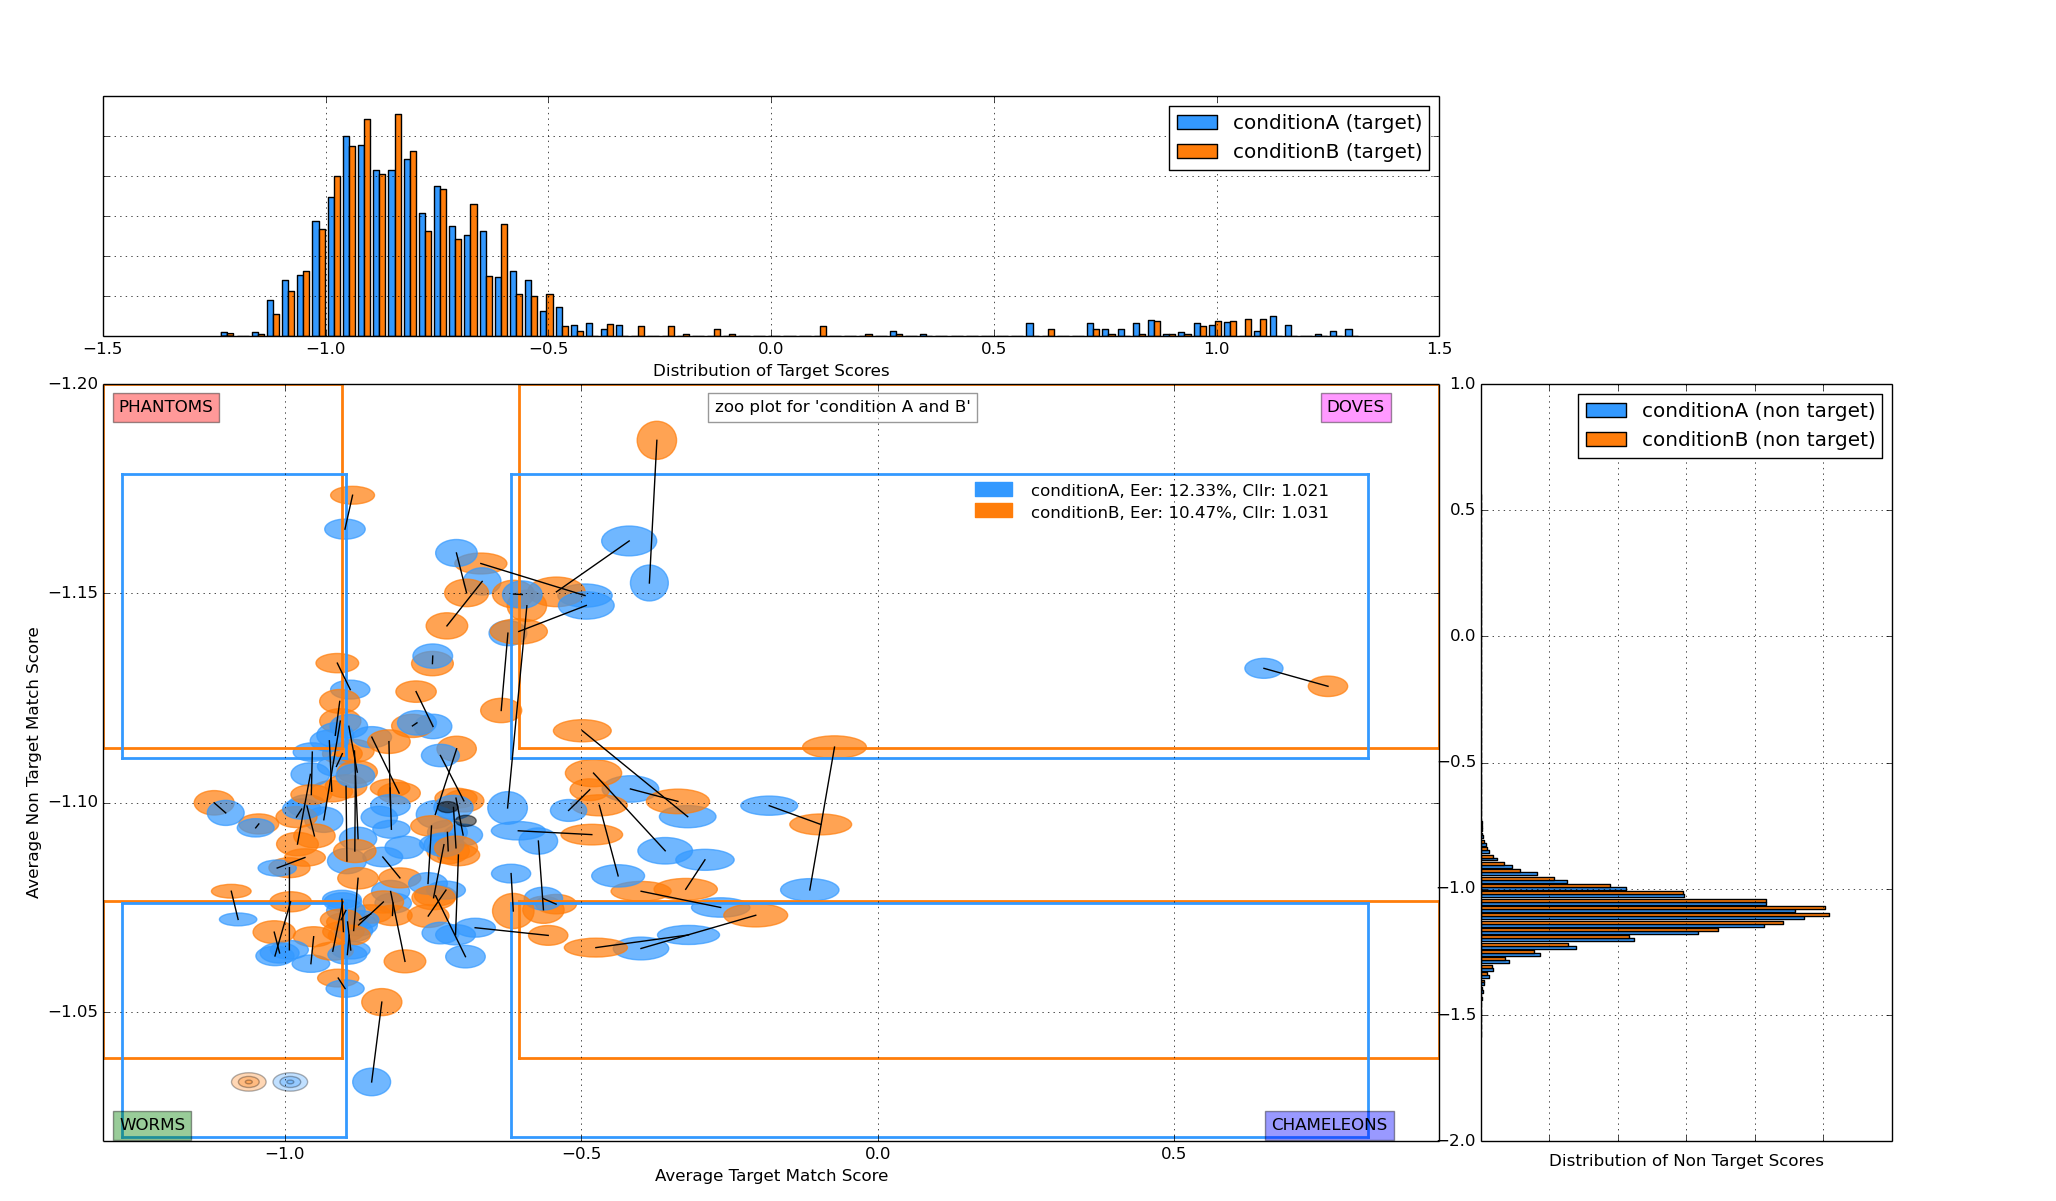
\includegraphics{images/A_and_B_zoo_plot.png}

The interface used to display the plots allows the user to zoom in on any part of the plots shown.

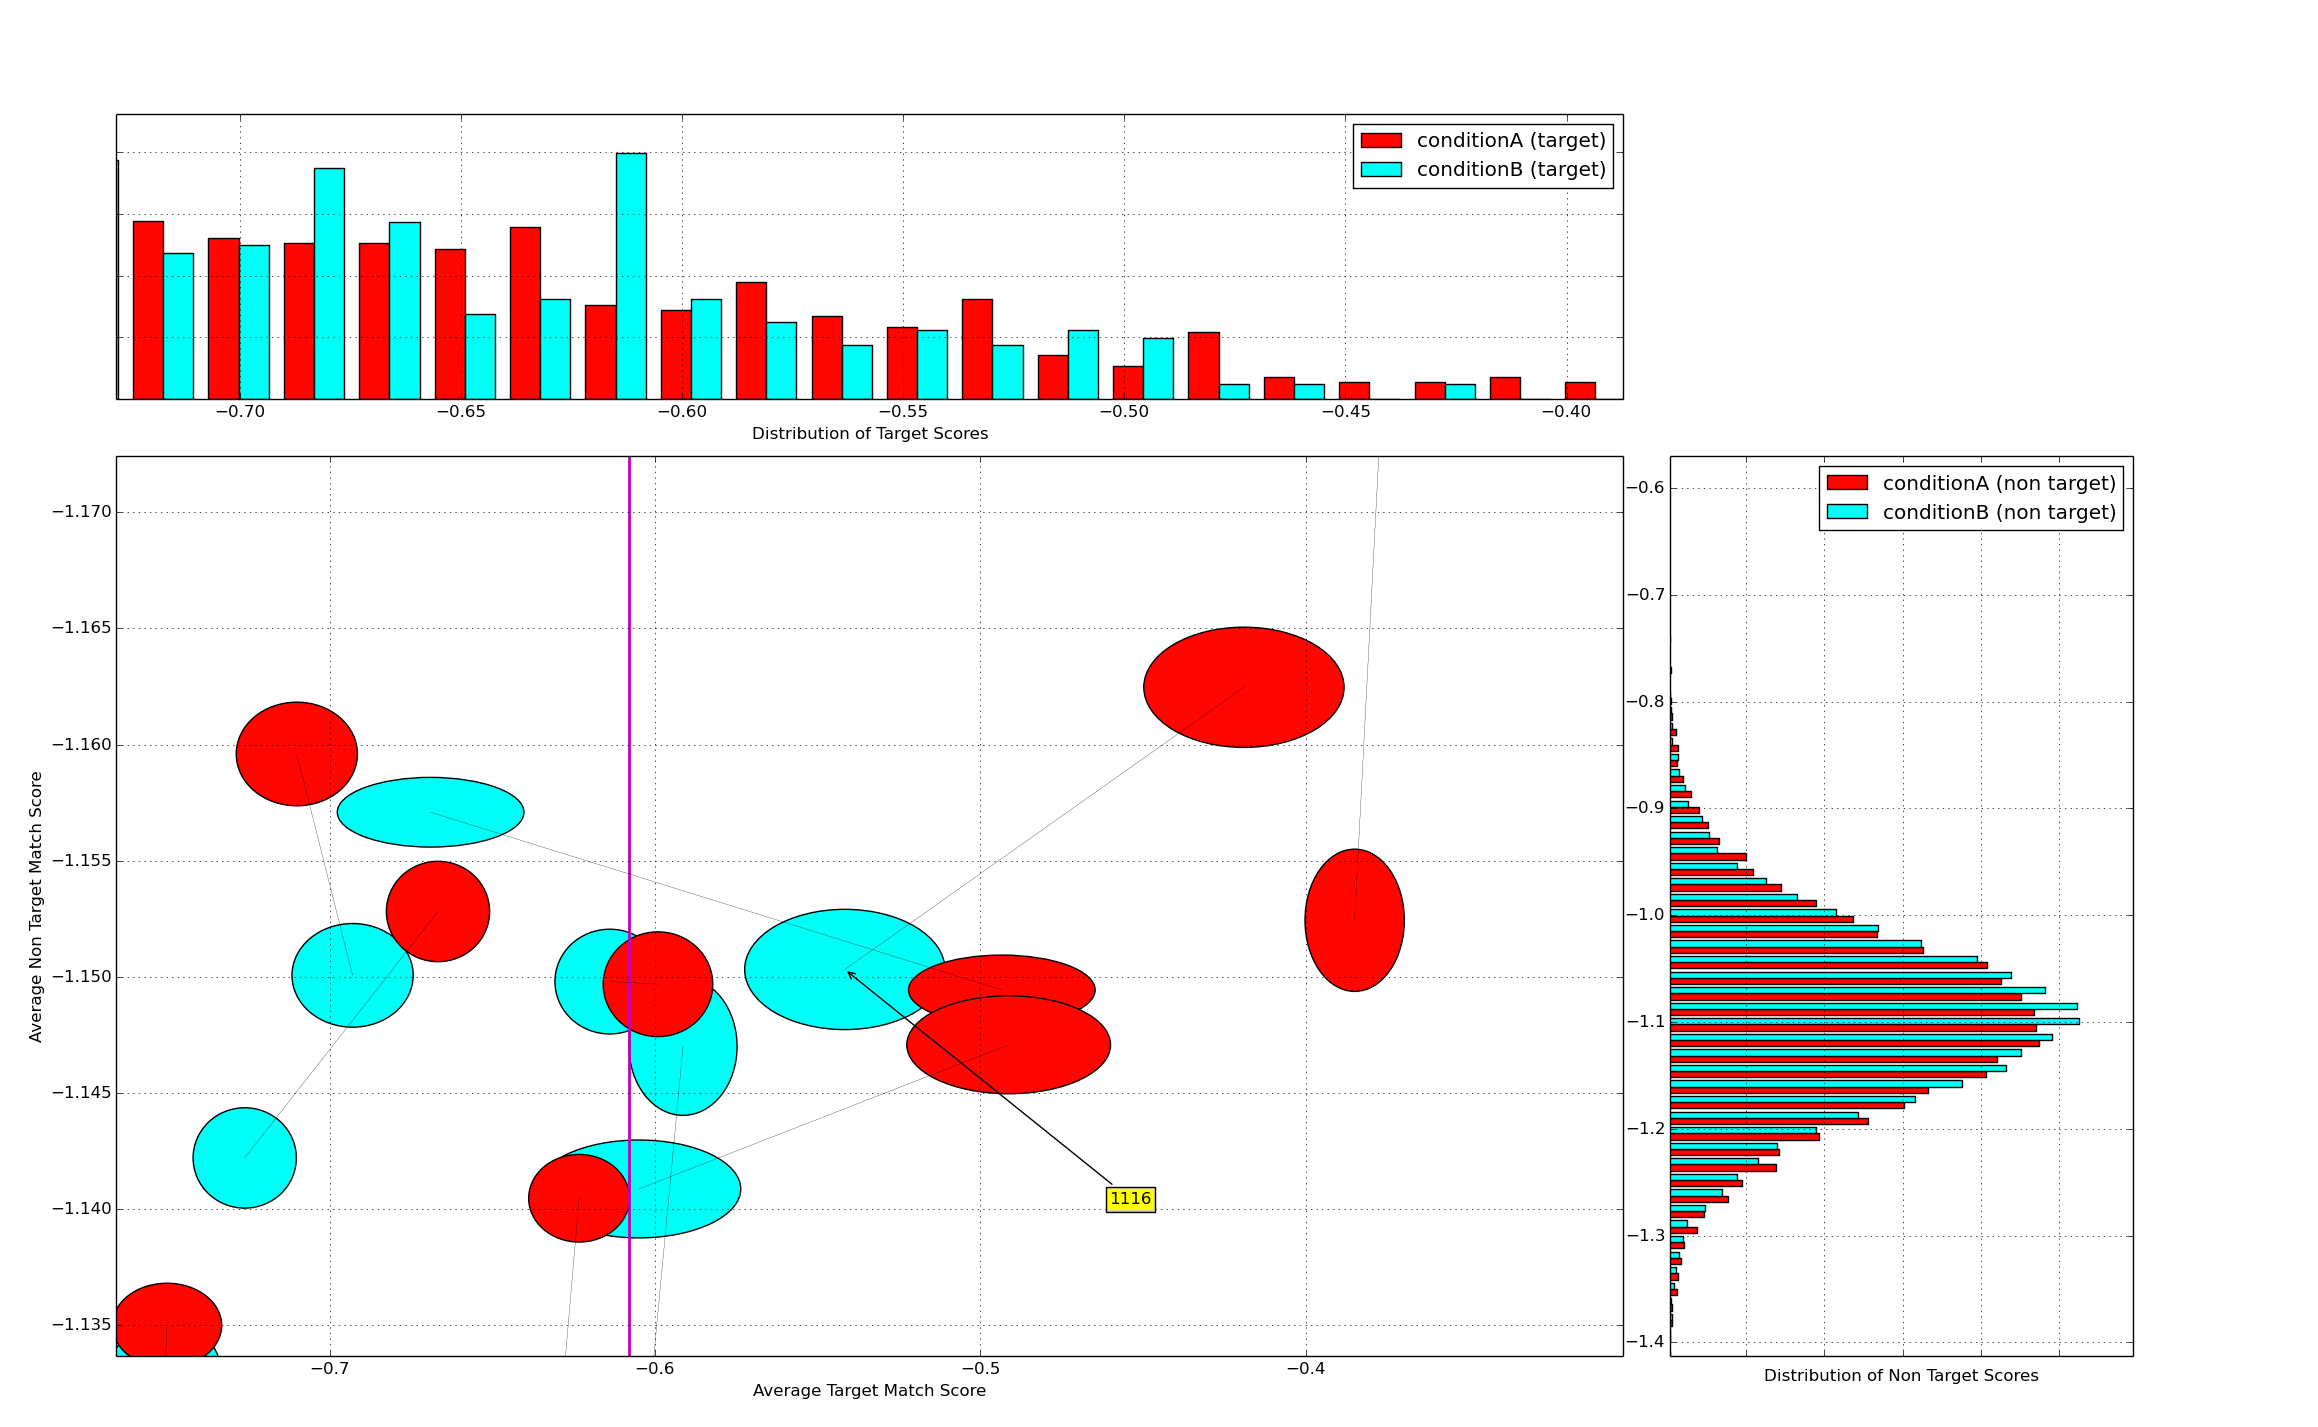
\includegraphics{images/condition_A_and_B_zoo_plot_zoom.png}


\chapter{Known Issues}
\label{issues:known-issues}\label{issues::doc}

\section{data separation character}
\label{issues:data-separation-character}
In data.py the following characters are used to group data: \_\#\_
If they are in your data set, e.g. as part of a label or meta data value, either change your data set or change the characters in format.py and choose non ambiguous replacements.


\section{matplotlib}
\label{issues:matplotlib}
The software works well with matplotlib-1.3.1. With older versions (like 0.99.3) you may encounter that plt.show(block=True) leads to an error message. Either upgrade matplotlib or change the statement to:

\begin{Verbatim}[commandchars=\\\{\}]
\PYG{n}{plt}\PYG{o}{.}\PYG{n}{show}\PYG{p}{(}\PYG{p}{)}
\end{Verbatim}


\chapter{bioplot.cfg}
\label{bioplot.cfg::doc}\label{bioplot.cfg:bioplot-cfg}
\begin{Verbatim}[commandchars=\\\{\}]
; This file contains flags and values used by bioplot.py
; All values here are defaults also contained in the program itself.
; You can use this file to change the program's default behaviour.
;
; Note: all options are CaSe sensitive !

; Copyright (C) 2014 Jos Bouten ( josbouten@gmail.com )

; This program is free software; you can redistribute it and/or modify
; it under the terms of the GNU General Public License as published by
; the Free Software Foundation; either version 2 of the License, or
; (at your option) any later version.

; This program is distributed in the hope that it will be useful,
; but WITHOUT ANY WARRANTY; without even the implied warranty of
; MERCHANTABILITY or FITNESS FOR A PARTICULAR PURPOSE.  See the
; GNU General Public License for more details.

; You should have received a copy of the GNU General Public License along
; with this program; if not, write to the Free Software Foundation, Inc.,
; 51 Franklin Street, Fifth Floor, Boston, MA 02110-1301 USA.


[cfg]
; If set to True 'allowDups' allows for both scores in a symmetric trial to be used.
; This means that the score of P vs Q and the score of Q vs P is used.
; Otherwise only the first encountered in the raw scores is used.
allowDups = False

; Choose a colormap: Spectral, gist\_ncar, hsv, gist\_rainbow or prism
colorMap = hsv

; set debug flag to True: will print a lot of info which might be of use
; when trying to debug the code.
debug = False

; Show config info at start of program on commandline
showConfigInfo = True

; Path to dir where results and plots are stored.
outputPath = output

; Are we running on OSX or not?
runningOSX = False

; Save all scores to text file separated in target and non target scores per meta value.
saveScores = True

[data]
; minimum value we expect for a score in type3 data.
minimum4Type3 = -1.0E+99
; maximum value we expect for a score in type3 data.
maximum4Type3 = 1.0E+99

; minimum value we expect for a score in type2 data.
minimum4Type2 = -1.0E+99
; maximum value we expect for a score in type2 data.
maximum4Type2 = 1.0E+99

; minimum value we expect for a score in type1 data.
minimum4Type1 = -1.0E+99
; maximum value we expect for a score in type1 data.
maximum4Type1 = 1.0E+99

[zoo]
; Show ellipses at position of data points representing standard deviation of target and non target scores
; as published by Alexander et al. @ IAFPA conference Zurich, Switserland, 2014
alexanderStyle = True

; Show labels for data points within quartile ranges
annotateQuartileMembers = True

; Add target and non target score histogram to zoo plot
boutenStyle = True

; Show histogram of shift of points depending on meta data values.
showCircularHistogram = True

; Show EER values
showEerValues = True

; Draw lines between labels with opposing metadata values
interconnectMetaValues = True

; Limit the std dev values of average non target and average target scores within +- 3 * std dev.
limitStdDevs = True

; When True will prevent the use of x-axis labels in the histograms added to the zoo plot.
noHistAnnot = False

; Opacity can be from 0 to 1 for small to large ellipses
; Restrict it to a portion of the range.
opacityLimitFactor = 0.85

; If we add labels to the command line, we dimm al the none matching points and
; ellipses by this factor thus making the given labels more prominent.
dimmingFactor = 0.8

; Scale data to screen resolution. 150 should be good for 1600x1024 ... 1280x1024
; Make smaller if you want bigger ellipses.
scaleFactor = 150

; Show all annotations when starting program; one click on the figure will make them disappear.
; Will only work if interconnectMetaValues is set to False.
showAnnotationsAtStartup = False

; Show reference ellipses or not.
showReference = True

; Do not show text with reference ellipses
showTextAtReferenceAtStartup = False

; Show kernel in zoo histogram
showKernelInHist = True

; Show mean of average target and non target points as a black dot.
showUnitDataPoint = True

; Give distinct colors to data points within quartile ranges. This is only done when the
; metadata field contains only one distinct value.
useColorsForQuartileRanges = True

; Big ellipses may overshadow smaller ones at the same position.
; Using opacity makes the smaller ones visible again.
useOpacityForBigEllipses = False

; Use vertical axis as proposed by Yager et al.
; When set to False the y-axis will be inversed.
yagerStyle = True

[layout]
; bottom\_h = left\_h = zleft + zwidth + spacing
; rectZoo = [zleft, zbottom, zwidth, zheight]
; rectHistx = [zleft, bottom\_h, zwidth, xheight]
; rectHisty = [left\_h, zbottom, ywidth, zheight]

; Left bottom x-position of zoo plot in boutenZoo
zLeft = 0.05

; Width of zoo plot
zWidth = 0.65

; Left bottom y-position of zoo plot in boutenZoo
zBottom = 0.05

; Height of zoo plot in boutenZoo
zHeight = 0.63

; Height of top histogram in boutenZoo
xHeight = 0.2

; Width of right hand side histogram in boutenZoo
yWidth = 0.2

; Spacing between zoo plot and left side of histograms in boutenZoo
spacing = 0.02

[histogram]
nrBins = 150

; Normalize histogram
normHist = True

; Show meta data values in histogram
showMetaInHist = True

[accuracy]
nrPoints = 100

[ranking]
nrPoints = 100

maxNrSteps = 100

[matrix]
; Not working at the moment:
; In the cross identification plot, we want at least
; this number of scores per label, otherwise skip
; the label.
; minNrScores4MatrixPlot = 25

; color map of the plot
matrixColorMap = Greys

; When set to True: combine matrices (if there are multiple
; because of different meta values) in a square or oblong matrix,
; otherwise make a horizontal bar or vertical column of matrices.
combineMatrices = True

; Show labels at tick marks
showMatrixLabels = True

; rotate xtick labels at a degree
labelAngle = 70

[probability]
; Number of threshold values used to calculate P(defense)
; and P(prosecution) from target and non target scores
; per meta value.
nrSamples4Probability = 500
\end{Verbatim}


\chapter{Indices and tables}
\label{index:indices-and-tables}\begin{itemize}
\item {} 
\emph{genindex}

\item {} 
\emph{modindex}

\item {} 
\emph{search}

\end{itemize}


\chapter{License}
\label{index:license}
Copyright (C) 2014 Jos Bouten ( \href{mailto:josbouten@gmail.com}{josbouten@gmail.com} )

This program is free software; you can redistribute it and/or modify
it under the terms of the GNU General Public License as published by
the Free Software Foundation; either version 2 of the License, or
(at your option) any later version.

This program is distributed in the hope that it will be useful,
but WITHOUT ANY WARRANTY; without even the implied warranty of
MERCHANTABILITY or FITNESS FOR A PARTICULAR PURPOSE.  See the
GNU General Public License for more details.

You should have received a copy of the GNU General Public License along
with this program; if not, write to the Free Software Foundation, Inc.,
51 Franklin Street, Fifth Floor, Boston, MA 02110-1301 USA.


\chapter{bioplot}
\label{index:bioplot}
You will not be able to use this program or any of its parts to slay a dragon, that
I'm sure of, and I do not guarantee that it is fit for any other purpose at all, but
I would appreciate if you would include a reference to this code and my name
in any publications you may write using it's features or add a source reference
to your code if you include some part(s) of this code in yours.

bioplot.py is a program which can draw several plots that can be used
when evaluating the performance of a biometric system. It reads settings from the file `bioplot.cfg'.
These settings may be used to determine the way information is shown in a plot, what directory plot files are written to etc.

The plot types currently supported are:
accuracy plot, cumulative score distribution plot, EER plot, histogram, matrix plot,
ranking plot, tippett plot and zoo plot.

Please read INSTALL.txt, this html documentation (note that the file `manual.txt' is obsolete) and bioplot.cfg before you try to use
`bioplot.py'. You'll learn more of the program's potential than from its command line help message.

@Windows dudes and dudettes: I'm afraid you have to run the program by hand from
a command line or build shortcuts which not only start the program but also
provide the command line options and parameters needed. You're on your
own here. I'm a command line junky anyway so I did not spend any
time building a gui. But don't fret. All plots ares shown in an interactive
window, you can click on that as much as you like. The interface
allows you to zoom in, click on a point to see the associated label, save
the plot in a file etc. etc.

What bioplot.py basically does is: read a data file and plot an interactive graph.
There is a choice to be made what type of graph you want.
The data has to be in a specific format. Actually there are 3 types of
format allowed. See `Data Files' below. All plots can be saved. This happens
automagically as well, but you get more useful results if this happens under
your control.

The program does a bit more than its command line arguments suggest.
You will notice this when you run it. It will for instance store all the
target and non target scores it distills from the data file you pass
to it and write them in text files (unless you set saveScores to False in bioplot.cfg). You can use these for further
processing. The experiment name you specify is used as part
of the filename: \textless{}exp\_name\textgreater{}\_\textless{}meta\_value\textgreater{}\_non\_target.txt, \textless{}exp\_name\textgreater{}\_\textless{}meta\_value\textgreater{}\_target.txt.
The files are stored in the directory specified by `outputPath' in
bioplot.cfg in it's {[}cfg{]} section. The default will be `output' in
the current directory. You can change this behaviour in bioplot.cfg via the following settings:

\begin{Verbatim}[commandchars=\\\{\}]
\PYG{p}{[}\PYG{n}{cfg}\PYG{p}{]}
\PYG{n}{outputPath} \PYG{o}{=} \PYG{n}{output}
\PYG{n}{saveScores} \PYG{o}{=} \PYG{n+nb+bp}{True}
\end{Verbatim}

If you run the program again using the same experiment
name, the scores are not saved anew, saving some processing time.
If you want to have new versions of these files, you need to delete
them before running bioplot.py again.

Next, if you choose to plot a zoo plot, the labels which fall within the
doves, chameleons, worms and phantom quartiles are saved in individual
text files: \textless{}exp\_name\textgreater{}\_chameleons.txt, \textless{}exp\_name\textgreater{}\_doves.txt,
\textless{}exp\_name\textgreater{}\_phantoms.txt and \textless{}exp\_name\textgreater{}\_worms.txt.
This automatically documents all outliers.

The labels with a standard deviation for their target scores or their
non target scores bigger than the unit standard deviation are stored
in a file \textless{}exp name\textgreater{}\_limited.txt together with the violating score (have a look
at the {\hyperref[zooplot:rst-zooplot]{\emph{Zoo plot}}} page for a general understanding of how the plot is made).

Example:

\begin{Verbatim}[commandchars=\\\{\}]
cat output/condition\_A\_limited.txt

1096 target std dev: 6.01978718893
335 non target std dev: 6.71906032808
\end{Verbatim}

Note that you can switch limiting on or off via setting limitStdDevs = False in bioplot.cfg section {[}zoo{]}.

Any plot you produce will be saved to disk as soon as you click on
the plot (to het the window focus) and press a key.
Note, it is important to maximise the plot's window to get a
proper layout of all elements in the plot! If you maximise and
press `s', you will be presented with a menu which will allow you
to save the plot anywhere you choose to.
If you press a different key, the plot will be saved locally in
the directory specified by outputPath.
This happens any time you press a key except l, k, g, s, f:

Note: l, k, g, s and f are predefined keys of the gui.
With them you can:

\begin{Verbatim}[commandchars=\\\{\}]
g: toggle grid on / off
k: toggle between lin horizontal scale and log horizontal scale
l: toggle between lin vertical scale and log vertical scale
s: open save menu
f: toggle between standard size and full screen
\end{Verbatim}

Any other key will make that the file is saved in its current dimensions.
To get a nice plot it is wise to maximise and then press any key. Then close
the window.


\chapter{Data files}
\label{index:data-files}
The command line allows to specify a filename and a type. The
default type is `type3' which corresponds to a text file with 7 fields. You need
not specify type3 as it is a default.
The type3 data file should contain data in a format like this example:

\begin{Verbatim}[commandchars=\\\{\}]
803742 17133729a.wav 80359 16842970b.wav 2.108616847991943 FALSE META\_VAL1
148407 47968376b.wav 89823 08087650a.wav 0.336018745422363 FALSE META\_VAL3
179408 34192626a.wav 80372 16749939b.wav 1.263523664188385 FALSE META\_VAL2
803442 48588750a.wav 80344 15560933b.wav 4.423274517059326 TRUE  META\_VAL2
\end{Verbatim}

Separation by comma's is also accepted.
This can be mixed as in:

\begin{Verbatim}[commandchars=\\\{\}]
803742,17133729a.wav,80359,16842970b.wav,2.108616847991943,FALSE,META\_VAL1
148407,47968376b.wav,89823,08087650a.wav,0.336018745422363,FALSE,META\_VAL3
179408 34192626a.wav 80372 16749939b.wav 1.263523664188385 FALSE META\_VAL2
803442,48588750a.wav,80344,15560933b.wav,4.423274517059326,TRUE, META\_VAL2
\end{Verbatim}

field 1: string: label identifying a person (training data)

field 2: string: name of data file containing biometric features or raw data originating from the person denoted by field 1 used for making a test model. In the example you see a wav-file, but this can be any string identifying a file or feature set.

field 3: string: label identifying a person (test data)

field 4: string: name of data file containing biometric features or raw data originating from the person denoted by field 3 used for training the reference model. In the example you see a wav-file, but this can be any string identifying a file or feature set.

field 5: string: floating point value: score of trial

field 6: string: meta data value for the experiment

Field 6 can be used to contrast scores of experiments in most plots.

So if you have 2 experiments where you change one variable, when doing a cross
identification test, the meta value can be used to group the experiment's scores.

E.g. you run an experiment with gender as the main variable an you collect scores of male
to male and female to female comparisons. You need to set the meta value for each score
accordingly. The meta value field allows bioplot to distinguish
between the two conditions and it will in essence plot 2 plots in one overview.
If the same label occurs on more than one occasion in the score list with different meta
values, then the points in a zoo plot with corresponding labels are interconnected
(see interconnectMetaValues setting in bioplot.cfg under {[}zoo{]}) . This makes it easy
to see what the effect of an individual label is when changing the experiment's condition.

Field 6 must be present. If you don't want to contrast experiments, then give all lines
the same meta value. Any string of characters (excluding white space) will do except
the special characters mentioned below under `Known Issues'.

File type `type2' is a variant of a file based data format:

\begin{Verbatim}[commandchars=\\\{\}]
62124-0 62124-1 0.383234709501  META\_VAL1
62124-0 62124-3 0.325683742762  META\_VAL1
62124-0 80491-2 0.239269435406  META\_VAL2
62124-0 64568-2 0.19219391048   META\_VAL1
62124-0 64568-3 0.125796630979  META\_VAL1
62124-0 77223-1 0.0895956531167 META\_VAL2
\end{Verbatim}

In this format basically format type3's field 1 and 2 are combined into the first field.
The same goes for type3's field 3 and 4, who are combined in field 2. You can use the corresponding code in data.py to adapt to your specific data file format OR write some code to map it to a type3 format file.

File `type1' is a database (sqlite) based data format and meant as an example on how to
use bioplot in combination with a database of scores. Specify `database' as filename on the
command line.

Example:

\begin{Verbatim}[commandchars=\\\{\}]
python ./bioplot.py -f database -t type1 -e 'data taken from db' -Z
\end{Verbatim}

You will have to adapt the query in the function \_readFromDatabase in data.py to your own needs.

There are 4 data files (of type3) which are meant as examples to play around
with: testdata\_A.txt, testdata\_B.txt, testdata\_C.txt and testdata\_ABC.txt

Example:

\begin{Verbatim}[commandchars=\\\{\}]
python ./bioplot.py -e "condition A" -f testdata\_A.txt -Z
\end{Verbatim}

If you experience any difficulties reading your data file, we can either discuss this
via email or you can send it to me ( \href{mailto:josbouten@gmail.com}{josbouten@gmail.com} ) so that I can have a look at it.
Please consider anonimizing the data before you send it to me by mail! Have a look at
anonimize.py and adapt it to your needs.

Finally:

If you have any questions or feature requests (no guarantees!) or find any bugs,
you can contact me at \href{mailto:josbouten@gmail.com}{josbouten@gmail.com}



\renewcommand{\indexname}{Index}
\printindex
\end{document}
